\graphicspath{%
{chapter1graph/}%
{chapter1graph/bg/}}
%\makeindex


\chapter{Distribution}

This chapter deals with concepts mainly related to various probability distribution.

\section{Probability Mass Function (PMF)}

The Probability Mass Function (PMF) gives the set of probabilities of \underline{discrete} outcome, e.g. discrete uniform PMF: roll one dice, each outcome is 1/6. \\

More formally, a probability mass function (PMF) is a function that gives the probability that a discrete random variable is exactly equal to some value. In Eqn. (\ref{binomialPMF}) below, the PMF gives the probability of getting exactly $k$ (discrete) successful Bernoulli trails. \\

Formal definition:\\
PMF is the probability distribution of a discrete random variable, and provides the possible values and associated probabilities. The probabilities associated with each possible values must be positive and sum up to 1. For all other values, the probabilities need to be 0.

\begin{figure}[h!]
\begin{center}
	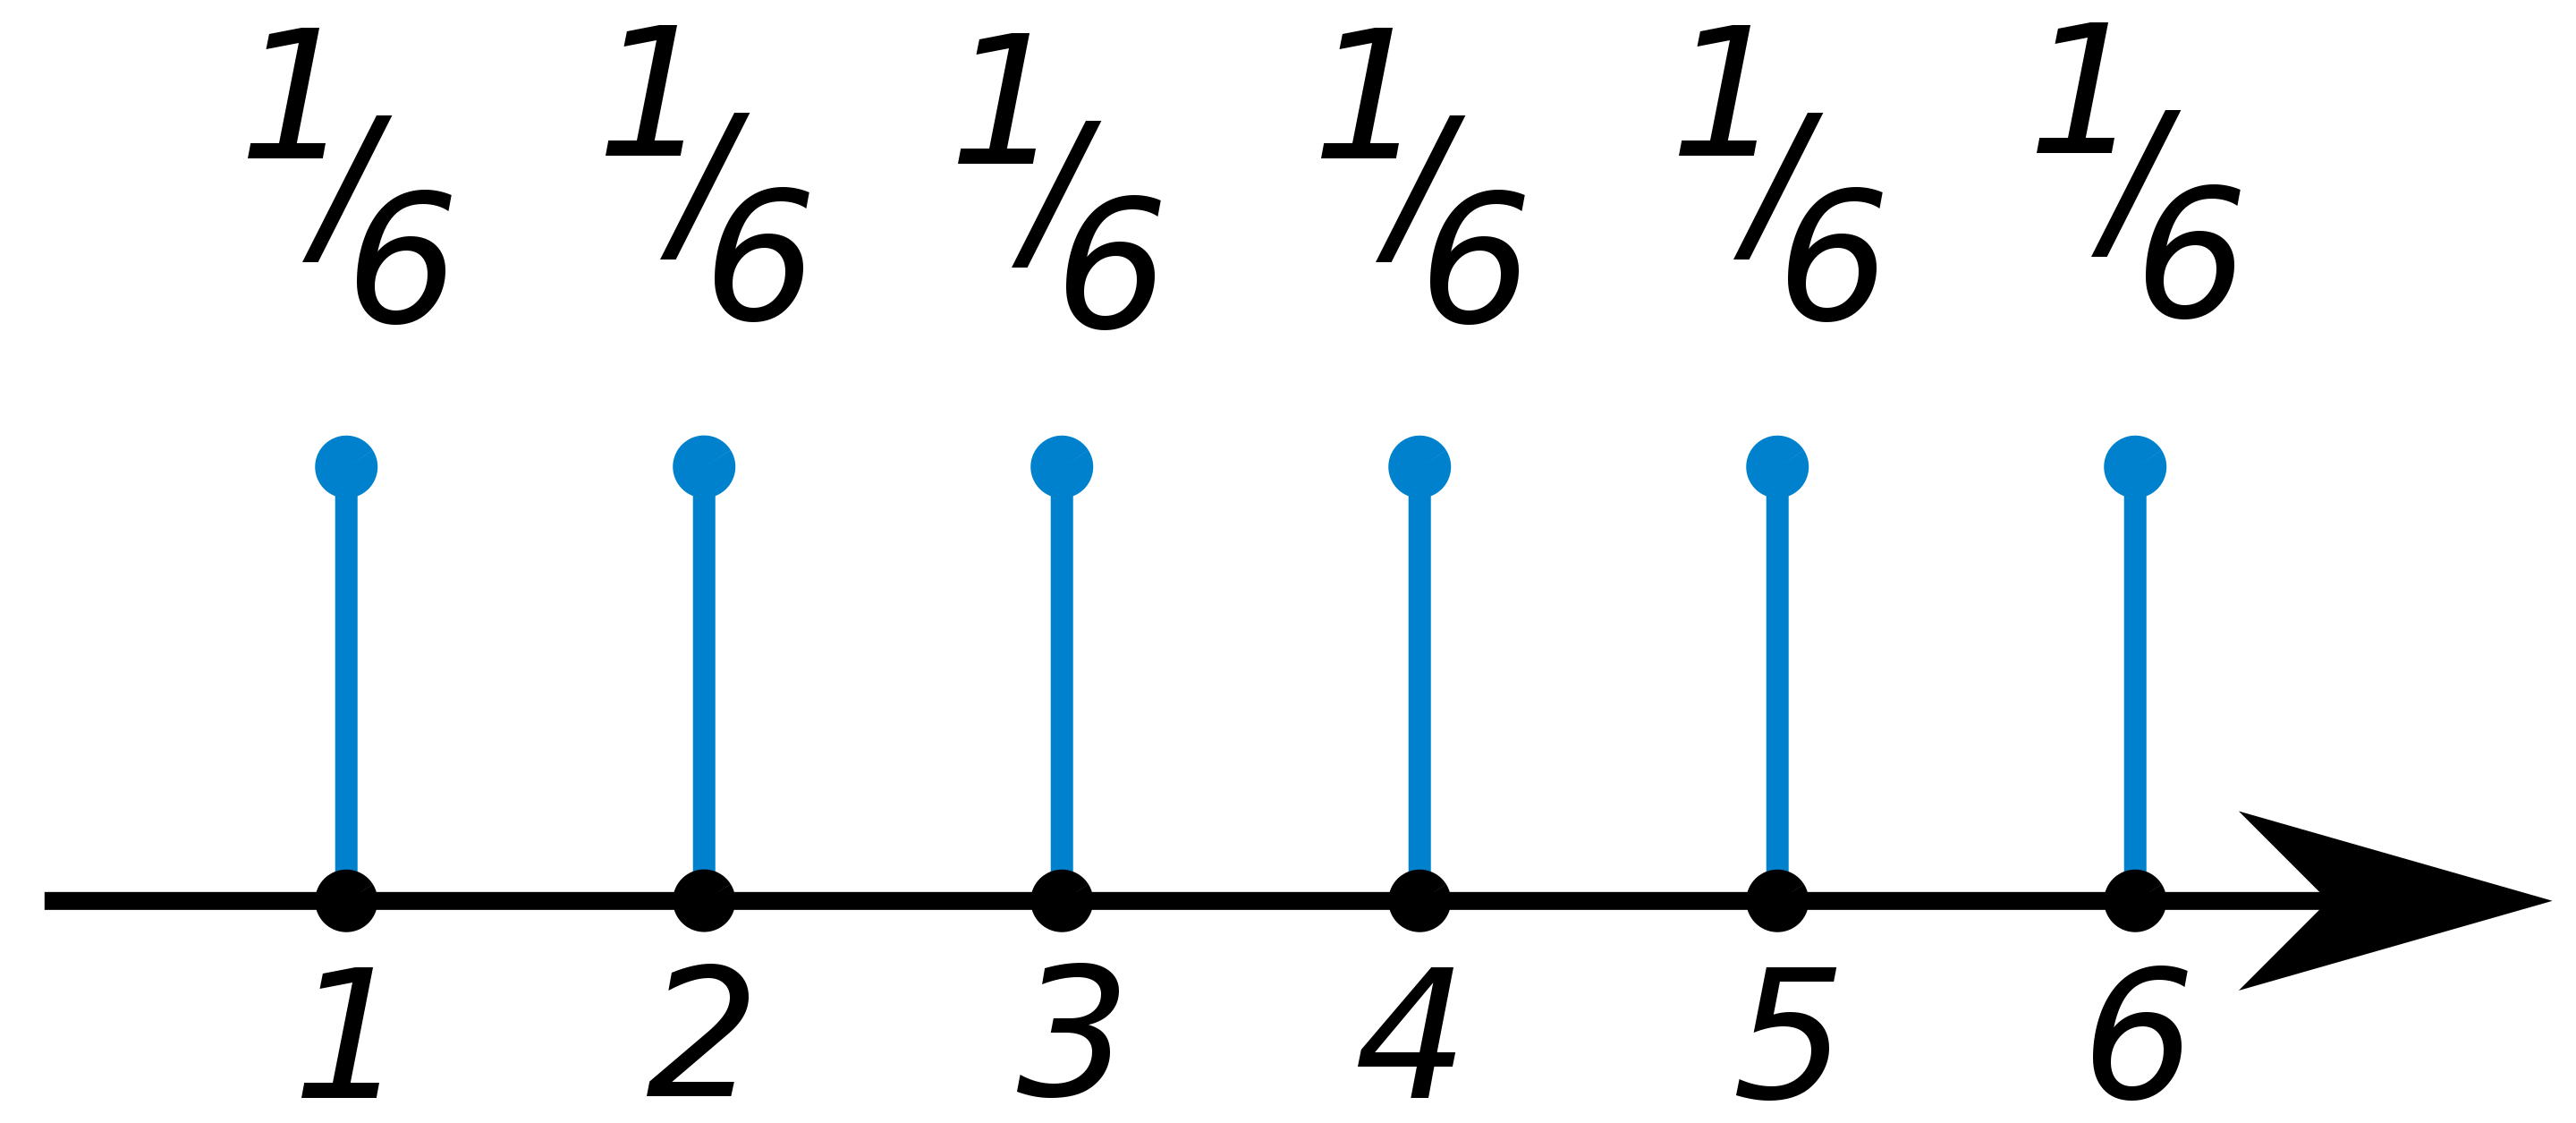
\includegraphics[scale=0.05]{Fair_dice_probability_distribution.png}
	\caption[]{The probability mass function of a fair die. All the values of this function must be non-negative and sum up to 1}
	\label{fairdiepmf}
	\end{center}
	\end{figure}

\section{Probability Density Function (PDF)}

The Probability Density Function (PDF) of a \underline{continuous} random variable, is a function whose value at any given sample (or point) in the sample space (the set of possible values taken by the random variable) can be interpreted as providing a relative likelihood that the value of the random variable would equal that sample. \\

In a more precise sense, the PDF is used to specify the probability of the random variable falling within a particular range of values, as opposed to taking on any one value. This probability is given by the integral of this variable's PDF over that range—that is, it is given by the area under the density function but above the horizontal axis and between the lowest and greatest values of the range. The probability density function is nonnegative everywhere, and its integral over the entire space is equal to 1. A PDF must be integrated over an interval to yield a probability, which is different from PMF (other than continuous VS discrete random variable).\\

More formally, the PDF is most commonly associated with absolutely continuous univariate distribution, a random variable $X$ has PDF $f_X$ and the probability of this variable taking values between $a$ and $b$, i.e. $a \le X \le b$ will be:
\begin{eqnarray}
P(a \le X \le b) = \int^{b}_{a} f_X (x) dx
\label{pdf}
\end{eqnarray}

If $F_X$ is the cumulative distribution function (CDF) of X, then:
\begin{eqnarray}
F_X(x) = \int^{x}_{-\infty} f_X(u) du
\label{cdf}
\end{eqnarray}

\begin{figure}[h!]
\begin{center}
	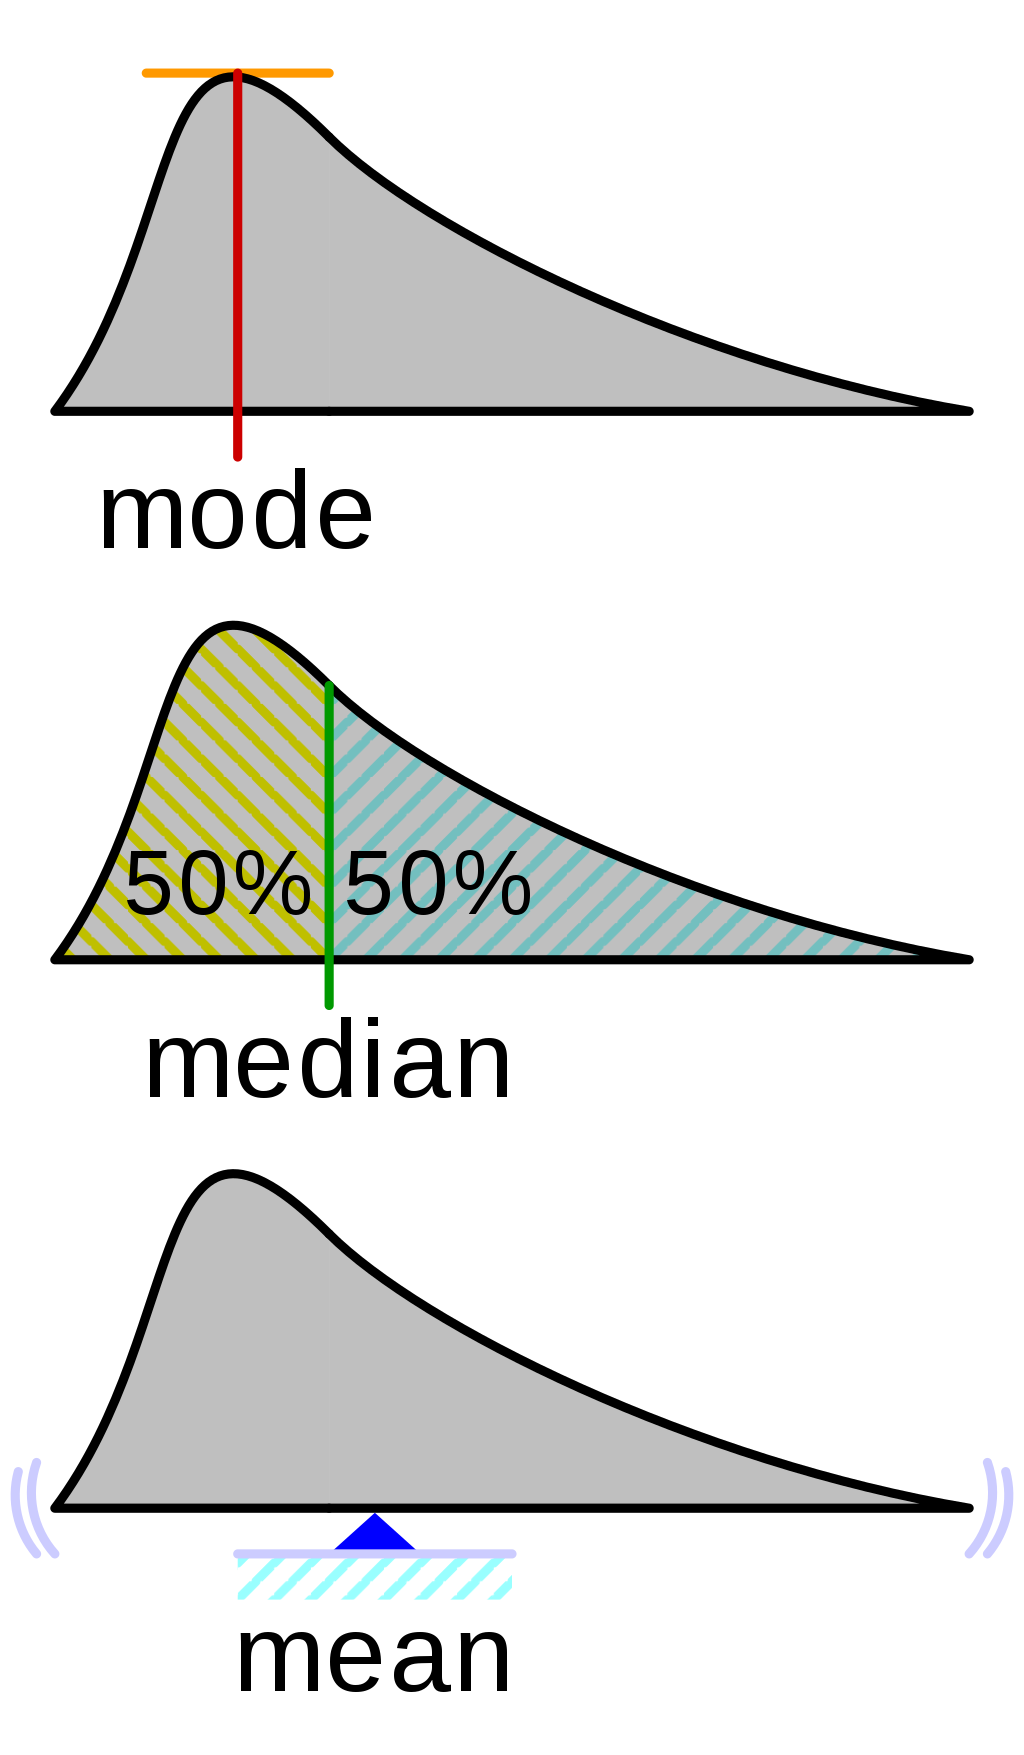
\includegraphics[scale=0.07]{pdf_visual.png}
	\caption[]{Geometric visualisation of the mode, median and mean of an arbitrary probability density function.}
	\label{fairdiepmf}
	\end{center}
	\end{figure}

\section{Cumulative Distribution Function (CDF)}

The Cumulative Distribution Function (CDF) of a real-valued random variable $X$ (continuous or discrete), evaluated at $x$, is the probability that $X$ will take a value less than or equal to $x$. In the case of a scalar continuous distribution, it gives the area under the probability density function (PDF) from $-\infty$ to $x$.

\section{Bernoulli Trials}

This is a \underline{random} experiment with exactly 2 possible outcomes. The probability of success is the same every time experiment is conducted. A similar analogy: Flipping a (possibly) biased coin, each coin has probability \textcolor{blue}{$p$} of landing heads (\textcolor{blue}{success}) and probability \textcolor{red}{$1 - p$} of landing tails (\textcolor{red}{failure}).  \\

Closely related to a Bernoulli trial is a binomial experiment, which consists of a fixed number $n$ of statistically independent Bernoulli trails, each with a probability of success \textcolor{blue}{$p$}, and counts the number of success. The number $k$ of success in $n$ Bernoulli trials is Binomially distributed. The probability of exactly $k$ success (out of $n$) is given by the probability mass function (PMF): 
\begin{eqnarray}
f(k,n,p) = P(k; n.p) =  P(X = k) = \binom{n}{k} p^k (1-p)^{n-k}
\label{binomialPMF}
\end{eqnarray}
where $\binom{n}{k}$ is the binomial coefficient:
\begin{eqnarray}
\binom{n}{k} = \frac{n !}{k! (n-k)!}
\label{binomialcoef}
\end{eqnarray}

Example:\\
Let's say a bank made 100 mortgage loans. It is possible that anywhere between 0 and 100 of the loans will be defaulted upon. You would like to know the probability of getting a given number of defaults, given that the probability of a default is $p = 0.05$. To investigate this, you will do a simulation. You will perform 100 Bernoulli trials. Here, a success is a default. (Remember that the word `success' just means that the Bernoulli trial evaluates to be True, i.e., did the loan recipient default?) You will do this for another 100 Bernoulli trials. And again and again until we have tried it 1000 times. Then, you will plot a histogram describing the probability of the number of defaults. So we have performed 1000 times of 100 mortgage trials, the histogram should show a maximum at about 5 (because $0.05 \times 100$) and probability is given in Eqn. (\ref{binomialPMF}). \\   

Example:\\
Consider the simple experiment where a fair coin is tossed four times. Find the probability that exactly two of the tosses result in heads.\\
\begin{eqnarray*}
P(2) &=& \binom{4}{2}p^2 (1-p)^{4-2} \\ 
&=& 6 \times (0.5)^2 \times (0.5)^2 \\ 
&=& \frac{3}{8}\\ 
\label{coin}
\end{eqnarray*}

When multiple Bernoulli trials are performed, each with its own probability of success, these are sometimes referred to as Poisson trials.

\section{Discrete variable: Binomial Distribution, Bin($n, p$)}

The Binomial Distribution with parameters $n$ and $p$, denoted Bin$(n,p)$ is the discrete probability distribution of the number of successes in a sequence of $n$ independent experiments, each asking a yes–no question, and each with its own boolean-valued outcome True (with probability $p$), or failure (with probability $q = 1- p$). A single success or failure experiment is also called a Bernoulli trial. \\

The binomial distribution is frequently used to model the number of successes in a sample of size $n$ drawn with replacement from a population of size $N$. If the sampling is carried out without replacement, then the draws are not independent and so the resulting distribution would be a hypergeometric distribution, not a binomial one. However, for N much larger than n, the binomial distribution remains a good approximation, and is widely used.

The PMF of Binomial Distribution is given in Eqn.(\ref{binomialPMF}). The CDF of Binomial Distribution can be expressed as:
\begin{eqnarray}
F(k; n, p) = P (X \le k) = \sum_{i=0}^{k} \binom{n}{i} p^i (1-p)^{n-i}
\label{binomialCDF}
\end{eqnarray}
where we just add up all the probability for all the previous $k$ values.

\section{Discrete variable: Bernoulli distribution, Ber($p$)}
The Bernoulli distribution is a special case of the binomial distribution, where a single trial is conducted (i.e., a binomial distribution with $n = 1$). The PMF of Bernoulli distribution, over possible outcomes $j$ is:
\begin{eqnarray}
f(k;p) = \begin{cases}
p,             \text{if $j$ = 1}\\
q = 1-p,      \text{if $j$ = 0}
\end{cases}
\end{eqnarray}

\section{Discrete variable: Geometric Distribution, Geo($p$)}

The Geometric Distribution is either of two discrete probability distribution described below: \\

1) The probability distribution of the number $X$ of Bernoulli Trials needed to get one success, supported on the set \{1, 2, 3, ... \}. \\

This geometric distribution, sometimes denoted $Geo(p)$, gives the probability that the \underline{first occurrence} of success requires $k$ independent trials, each with success probability (Bernoulli Trial). The Probability Mass Function (PMF) is (probability that the $k$th trial (out of $k$ trials) is the first success):\\
\begin{eqnarray}
P(X=k) = (1 - p)^{k-1} p, k=1,2,3,...
\label{geo_pmf_1}
\end{eqnarray}

and the Cumulative Distribution Function (CDF) is:\\
\begin{eqnarray}
P(X \le k) = 1 - (1-p)^k
\label{geo_cdf_1}
\end{eqnarray}

This distribution is used for modelling the number of trials up to and including the first success.

2) The probability distribution of the number $Y = X - 1$ of failures before the first success, supported on the set \{0, 1, 2, 4, ... \}. \\

This form of geometric distribution is used for modelling the number of failures until the first success:

\begin{eqnarray}
P(X=k) = (1 - p)^k p, k=0,1,2,3,...
\label{geo_pmf_2}
\end{eqnarray}

and the Cumulative Distribution Function (CDF) is:\\
\begin{eqnarray}
P(X \le k) = 1 - (1-p)^{k+1}
\label{geo_cdf_2}
\end{eqnarray}

The geometric distribution is an appropriate model if the following assumption is true:\\
1) The phenomenon being  modelled is a sequence of independent trials.\\
2) There are only two possible outcomes for each trial. \\
3) The probability of success $p$ is the same for each trial.\\

\begin{figure}[h!]
\begin{center}
	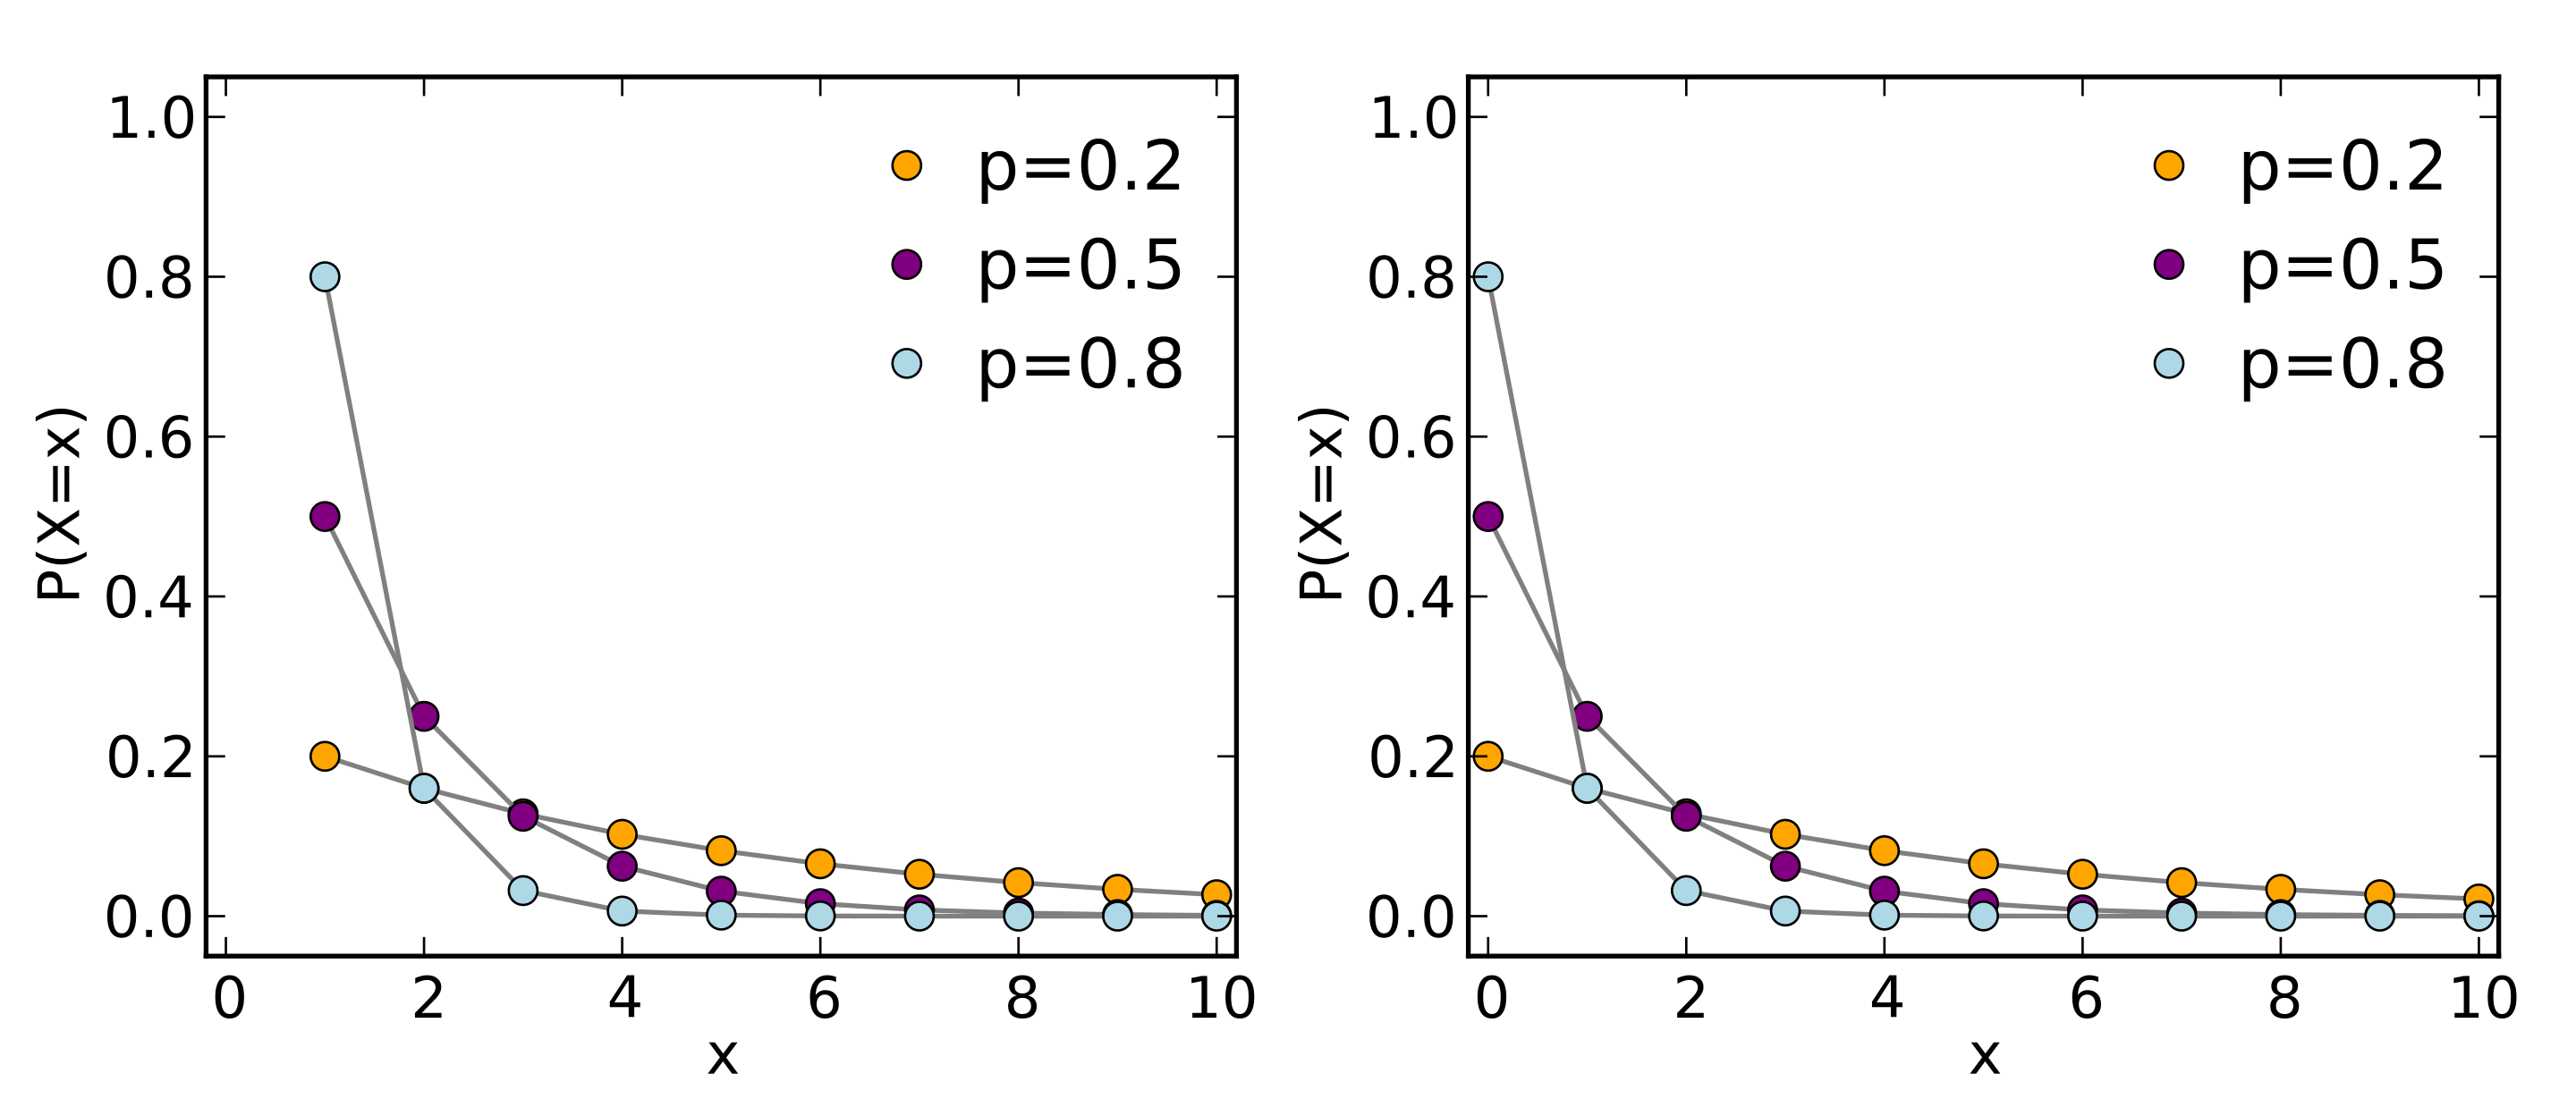
\includegraphics[scale=0.09]{geometric_pmf.png}
	\caption[]{Probability Mass Function (PMF) of geometric distribution for case 1) (left) and case 2) (right).}
	\label{fairdiepmf}
	\end{center}
	\end{figure}
	
\begin{figure}[h!]
\begin{center}
	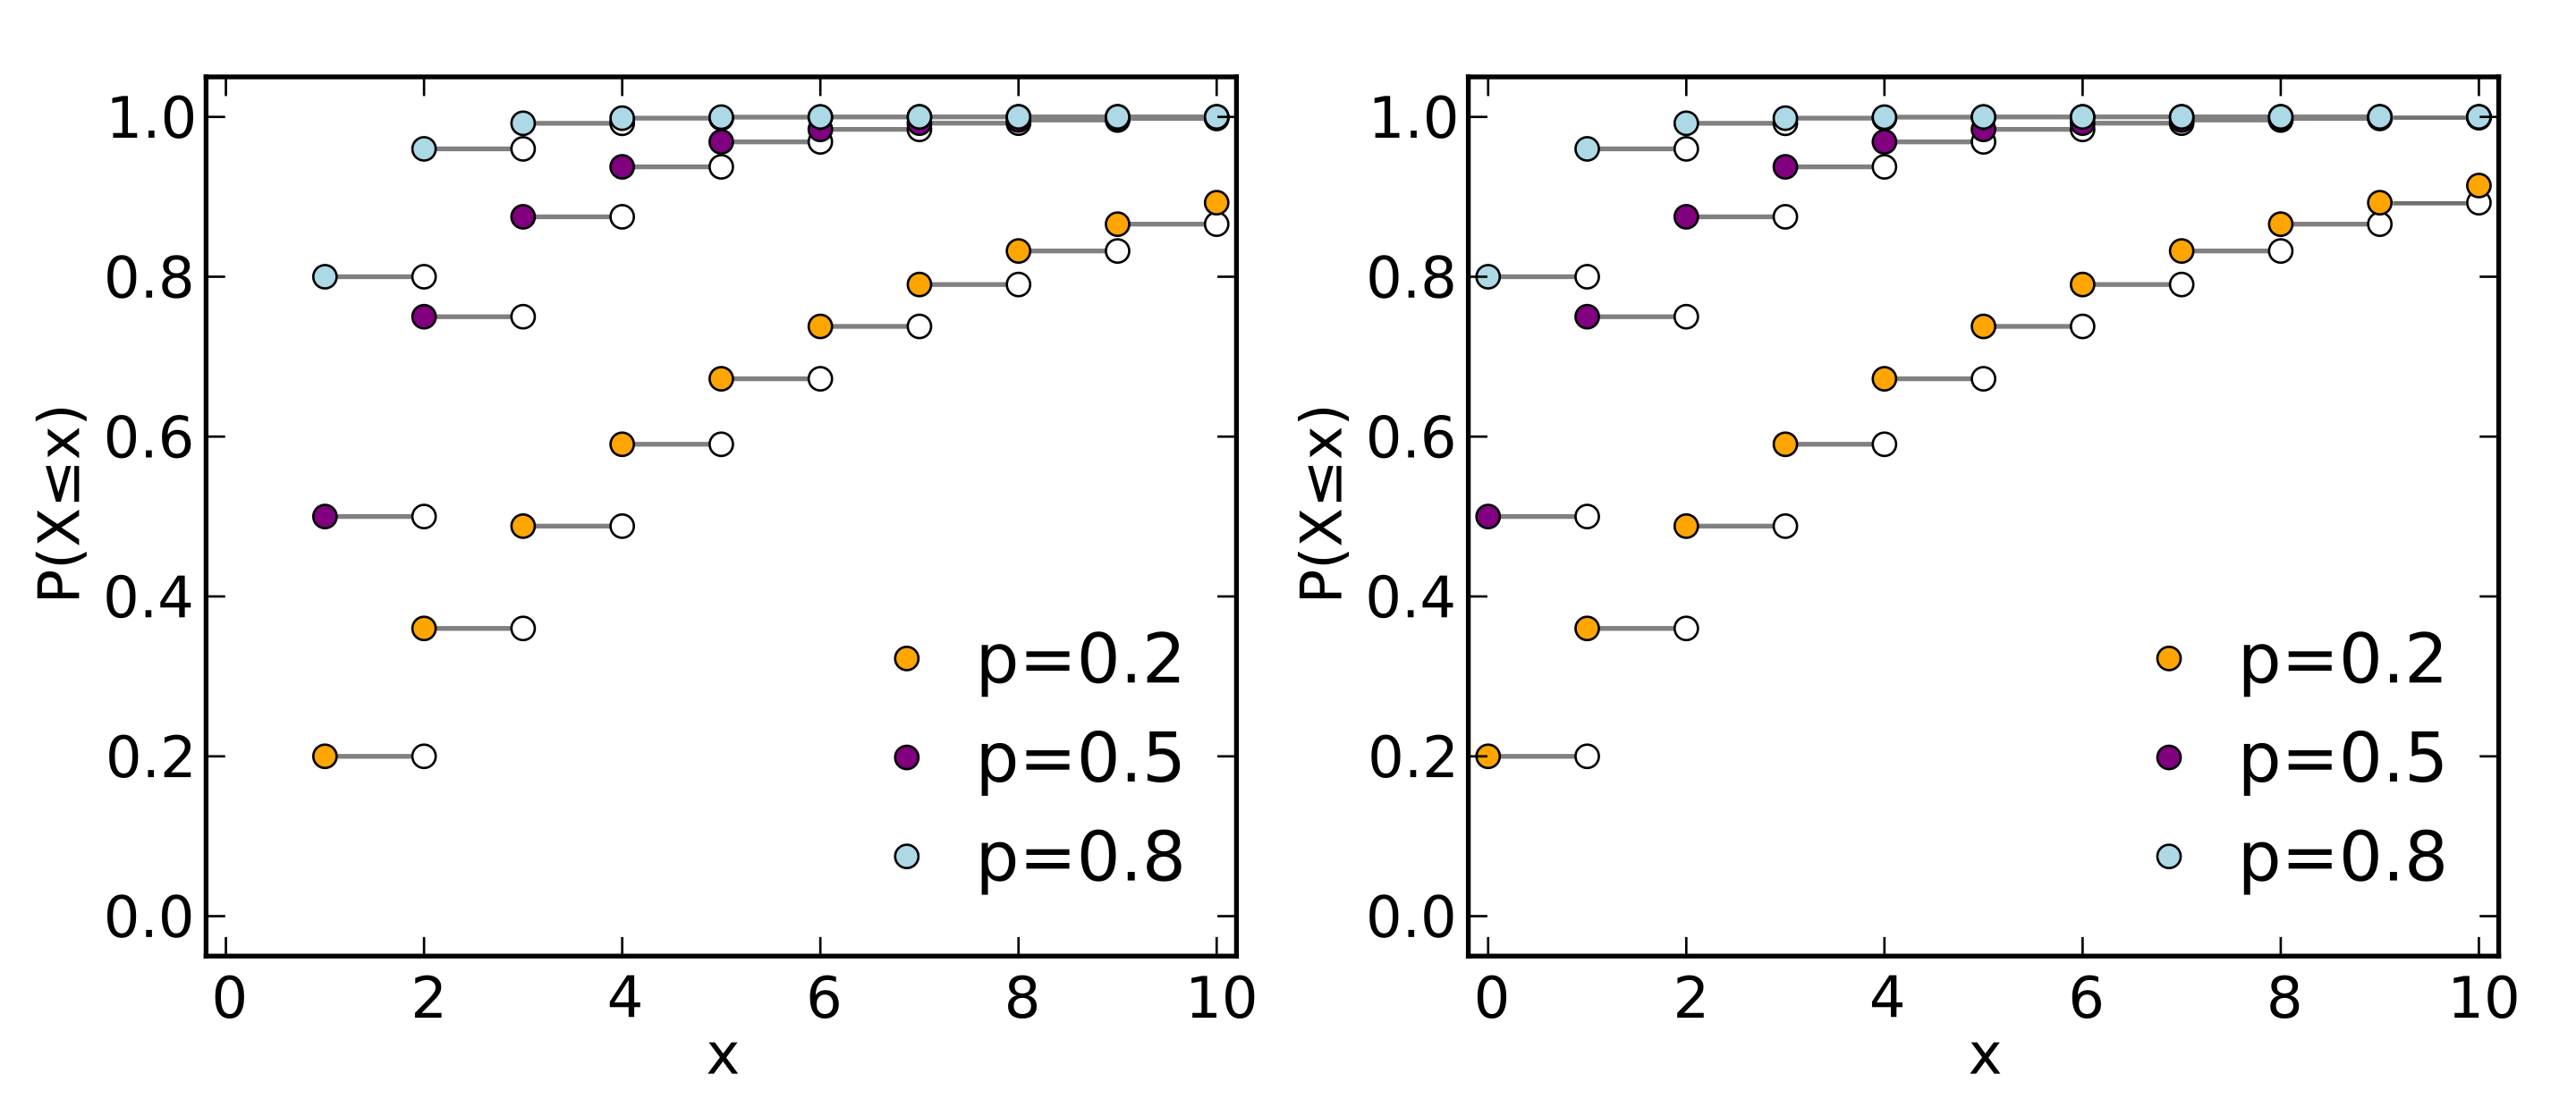
\includegraphics[scale=0.09]{geometric_cdf.png}
	\caption[]{Cumulative Distribution Function (CDF) of geometric distribution for case 1) (left) and case 2) (right).}
	\label{fairdiepmf}
	\end{center}
	\end{figure}

\section{Discrete variable: Poisson Distribution, Pois($\lambda$)}

The Poisson Distribution is a discrete probability distribution that expresses the probability of a given number of events occurring in a fixed interval of times or space if these events occur with a known constant mean rate and independently of the time since the last event. \\

For instance, an individual keeping track of the amount of mail they receive each day may notice that they receive an average number of 4 letters per day. If receiving any particular piece of mail does not affect the arrival times of future pieces of mail, i.e., if pieces of mail from a wide range of sources arrive independently of one another, then a reasonable assumption is that the number of pieces of mail received in a day obeys a Poisson distribution. \\

The Poisson Distribution is popular for modelling the number of times an event occurs in an interval of time or space. A discrete random variable $X$ is said to have a Poisson Distribution with parameter $\lambda > 0$, if, for $k = 0,1,2, ...$, the Probability Mass Function (PMF) of $X$ is given by:
\begin{eqnarray}
f(k;\lambda) = P(X=k) = \frac{\lambda^k e^{- \lambda}}{k !} = P(\text{k events in interval})
\label{poisson_pmf}
\end{eqnarray}
where $\lambda$ is equal to the expected value of $X$ and also its variance.\\

The Cumulative Distribution Functions (CDF) is:
\begin{eqnarray}
F(k;\lambda) = e^{- \lambda} \sum^{k}_{i=0} \frac{\lambda^i}{i !}
\label{poisson_cdf}
\end{eqnarray}

The Poisson Distribution is an appropriate model if the following assumptions are true: \\
1) $k$ is the number of times an event occurs in an interval and k can take values 0, 1, 2, ...\\
2) The occurrence of one event does not affect the probability that a second event will occur. That is, events occur independently.\\
3) The average rate at which events occur is independent of any occurrences. For simplicity, this is usually assumed to be constant, but may in practice vary with time.\\
4) Two events cannot occur at exactly the same instant; instead, at each very small sub-interval exactly one event either occurs or does not occur.\\

The Poisson Distribution is also the limit of a binomial distribution, , for which the probability of success $p$ for each trial equals to $\frac{\lambda}{\text{num. of trials}}$, as the number of trials goes to infinity. \\
If the number of Bernoulli trials goes to infinity (or every large), then Binomial distribution can be converted into Poisson distribution. ($p$ will be small, it is a rare event.)

\begin{figure}[h!]
\begin{center}
	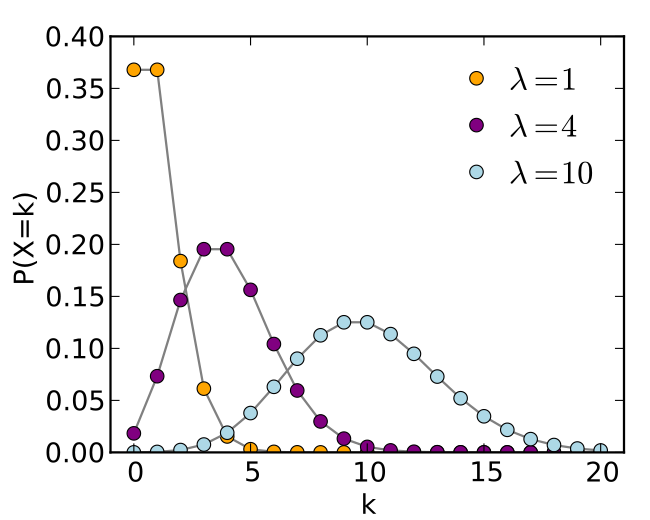
\includegraphics[scale=0.25]{poisson_pmf.png}
	\caption[]{Probability Mass Function (PMF) of Poisson distribution.}
	\label{fairdiepmf}
	\end{center}
	\end{figure}
	
\begin{figure}[h!]
\begin{center}
	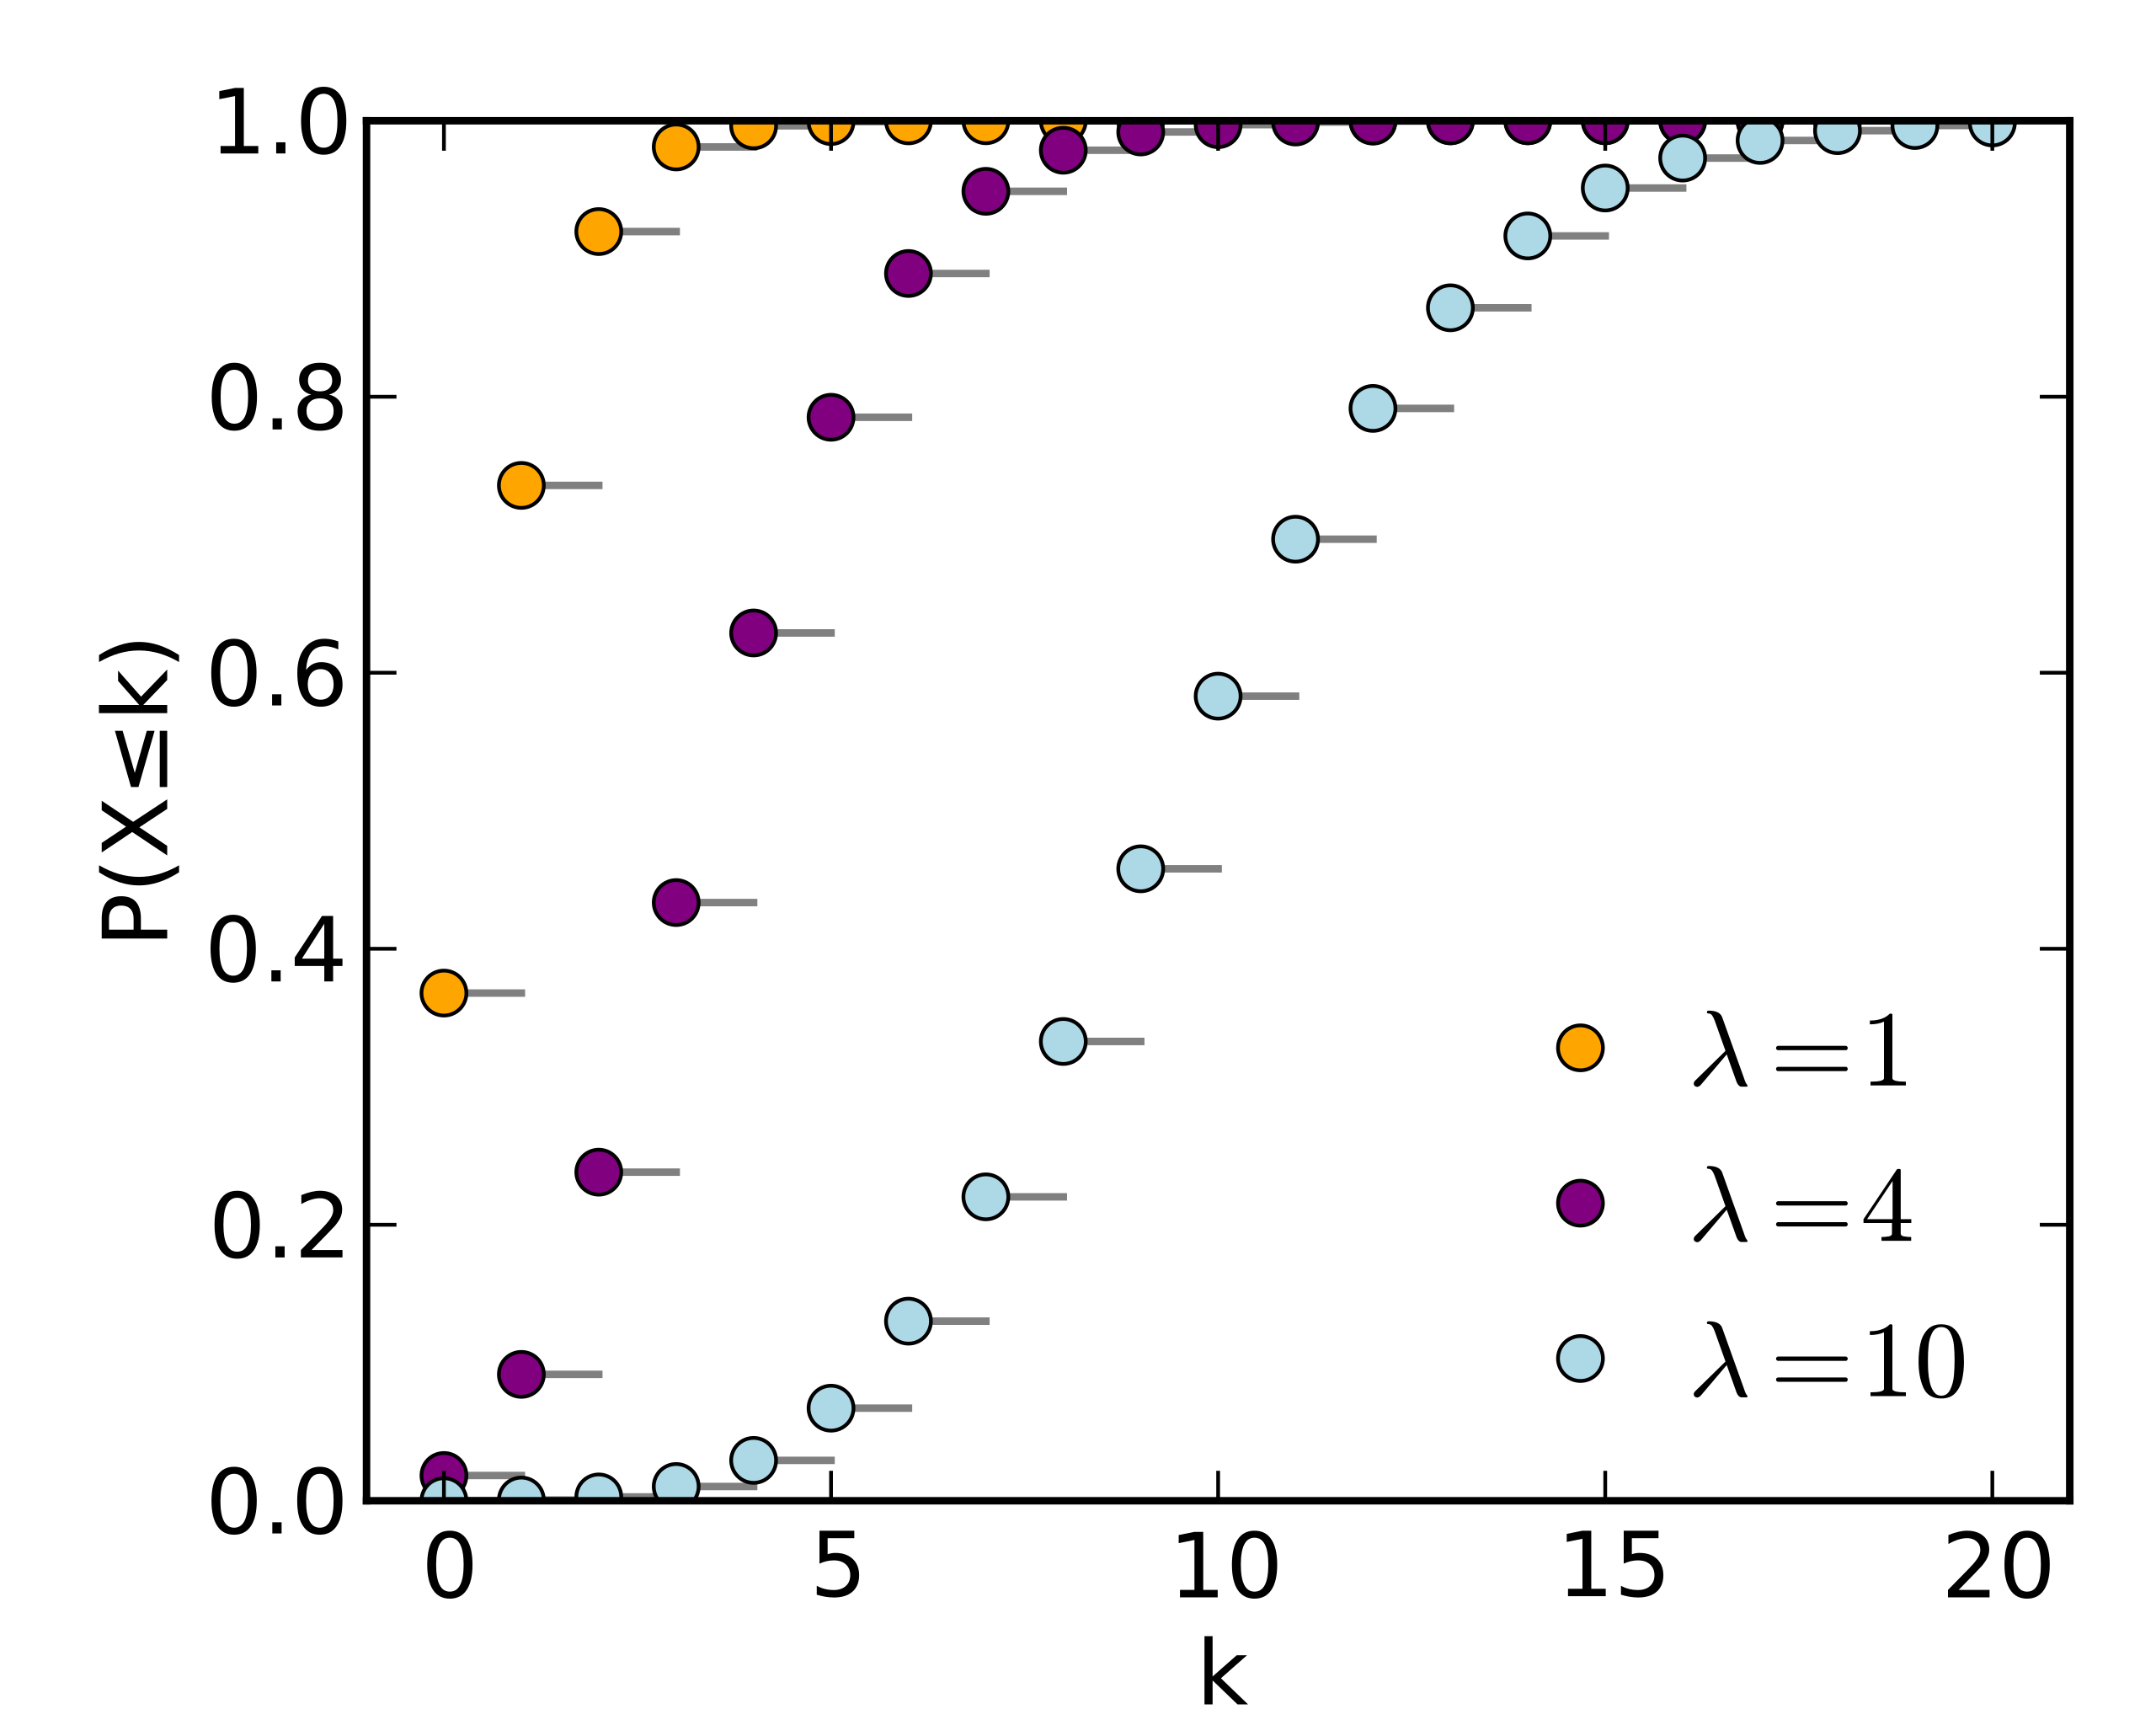
\includegraphics[scale=0.07]{poisson_cdf.png}
	\caption[]{Cumulative Distribution Function (CDF) of Poisson distribution.}
	\label{fairdiepmf}
	\end{center}
	\end{figure}
	
\section{Continuous variable: Normal Distribution, $\mathcal{N}(\mu, \sigma^2)$}

A Normal (Gaussian) distribution is a type of continuous probability distribution for a real-valued random variable. The general form of its Probability Density Function (PDF) is:
The Cumulative Distribution Functions (CDF) is:
\begin{eqnarray}
f(x) = \frac{1}{\sigma \sqrt{2 \pi}} e^{-\frac{1}{2}(\frac{x-\mu}{\sigma})^2}
\label{normal_pdf}
\end{eqnarray}
where $\mu$ is the mean or expectation of the distribution (and also its median and mode), while $\sigma$ is the standard deviation. The variance of the distribution is $\sigma^2$.  Note that these $\mu$ and $\sigma$ is associated with Normal Distribution and not the one computed directly from the data. Note also that Normal Distribution are affected by outliers because probability of any event happen more than 4 standard deviations from the mean is very low. \\

Normal distributions are often used in the natural and social sciences to represent real-valued random variables whose distributions are not known. Their importance is partly due to the Central Limit Theorem (CLT). CLT establishes that in some situations, when independent random variables are added, their properly normalized sum tends toward a normal distribution (informally a bell curve), even if the original variables themselves are not normally distributed. \\

The Cumulative Distribution Function (CDF) for Normal Distribution is:
\begin{eqnarray}
F(x) = \frac{1}{2}[1 + \text{erf} \; (\frac{x - \mu}{\sigma \sqrt{2}})]
\label{normal_cdf}
\end{eqnarray}
where erf is the error function defined as:
\begin{eqnarray}
\text{erf} \; z = \frac{2}{\sqrt{\pi}} \int^{z}_{0} e^{-t^2} dt
\label{errfunc}
\end{eqnarray}

\begin{figure}[h!]
\begin{center}
	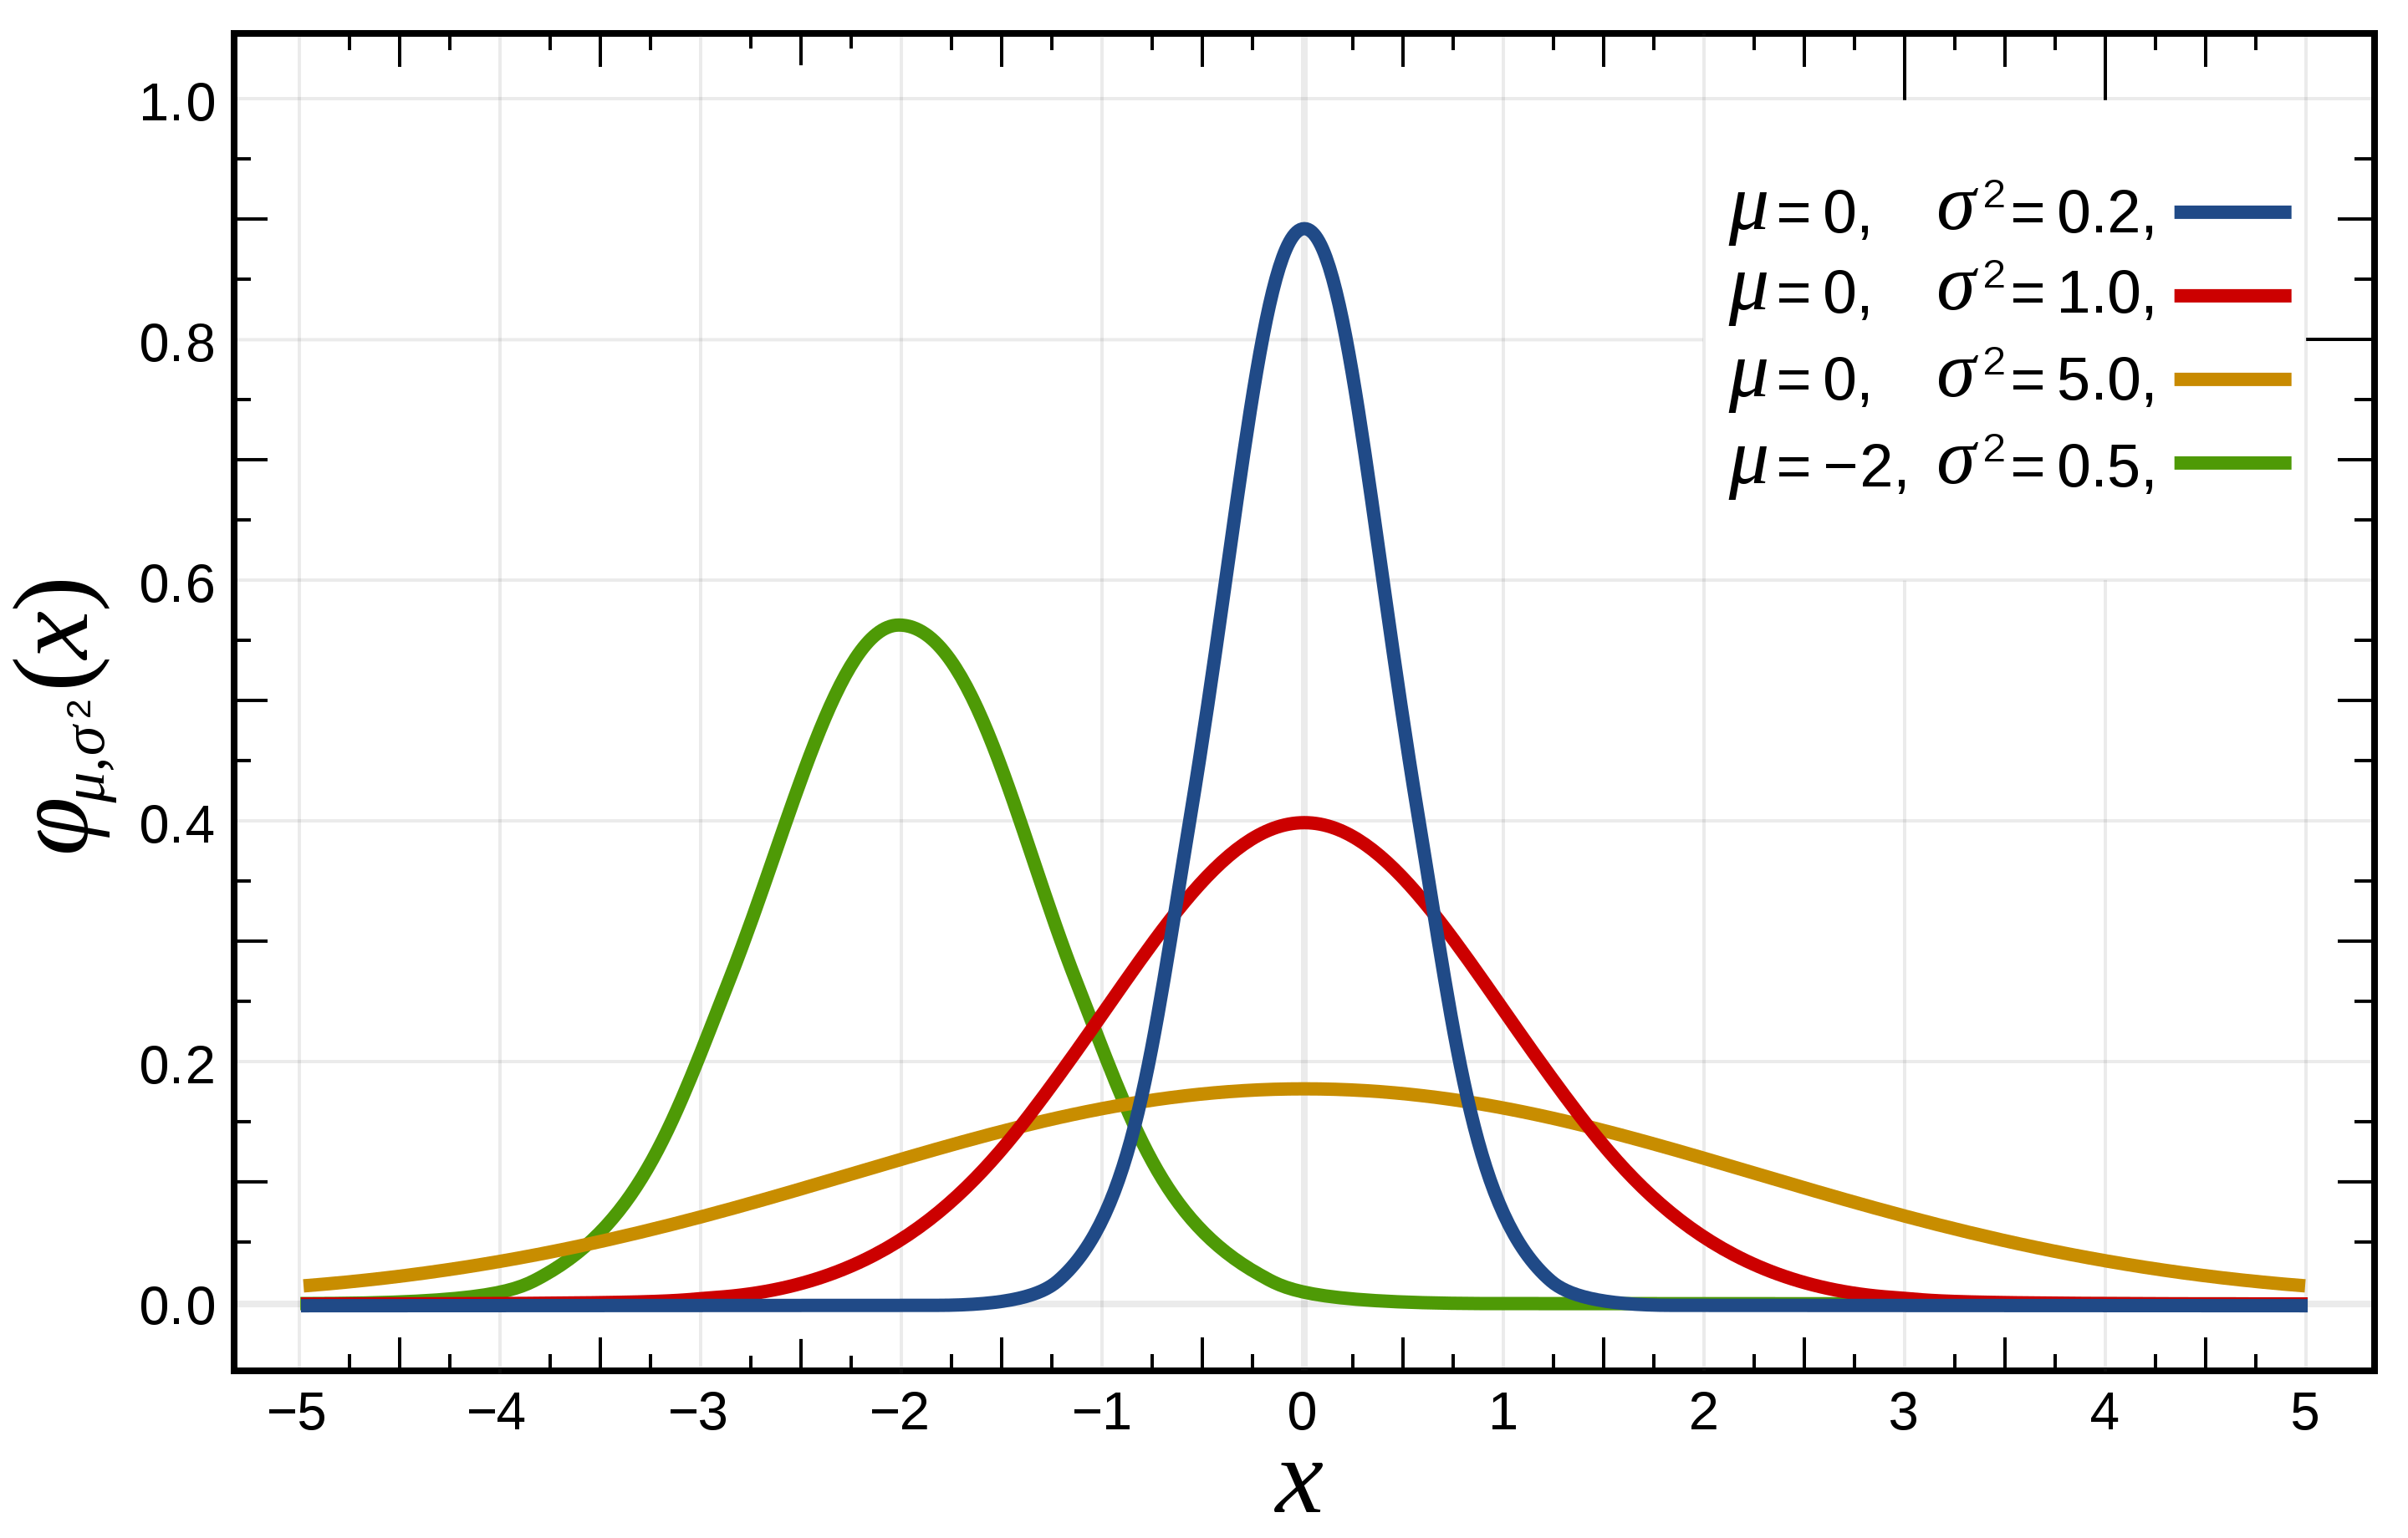
\includegraphics[scale=0.08]{normal_pdf.png}
	\caption[]{Probability Density Function (PDF) of Normal distribution.}
	\label{fairdiepmf}
	\end{center}
	\end{figure}
	
\begin{figure}[h!]
\begin{center}
	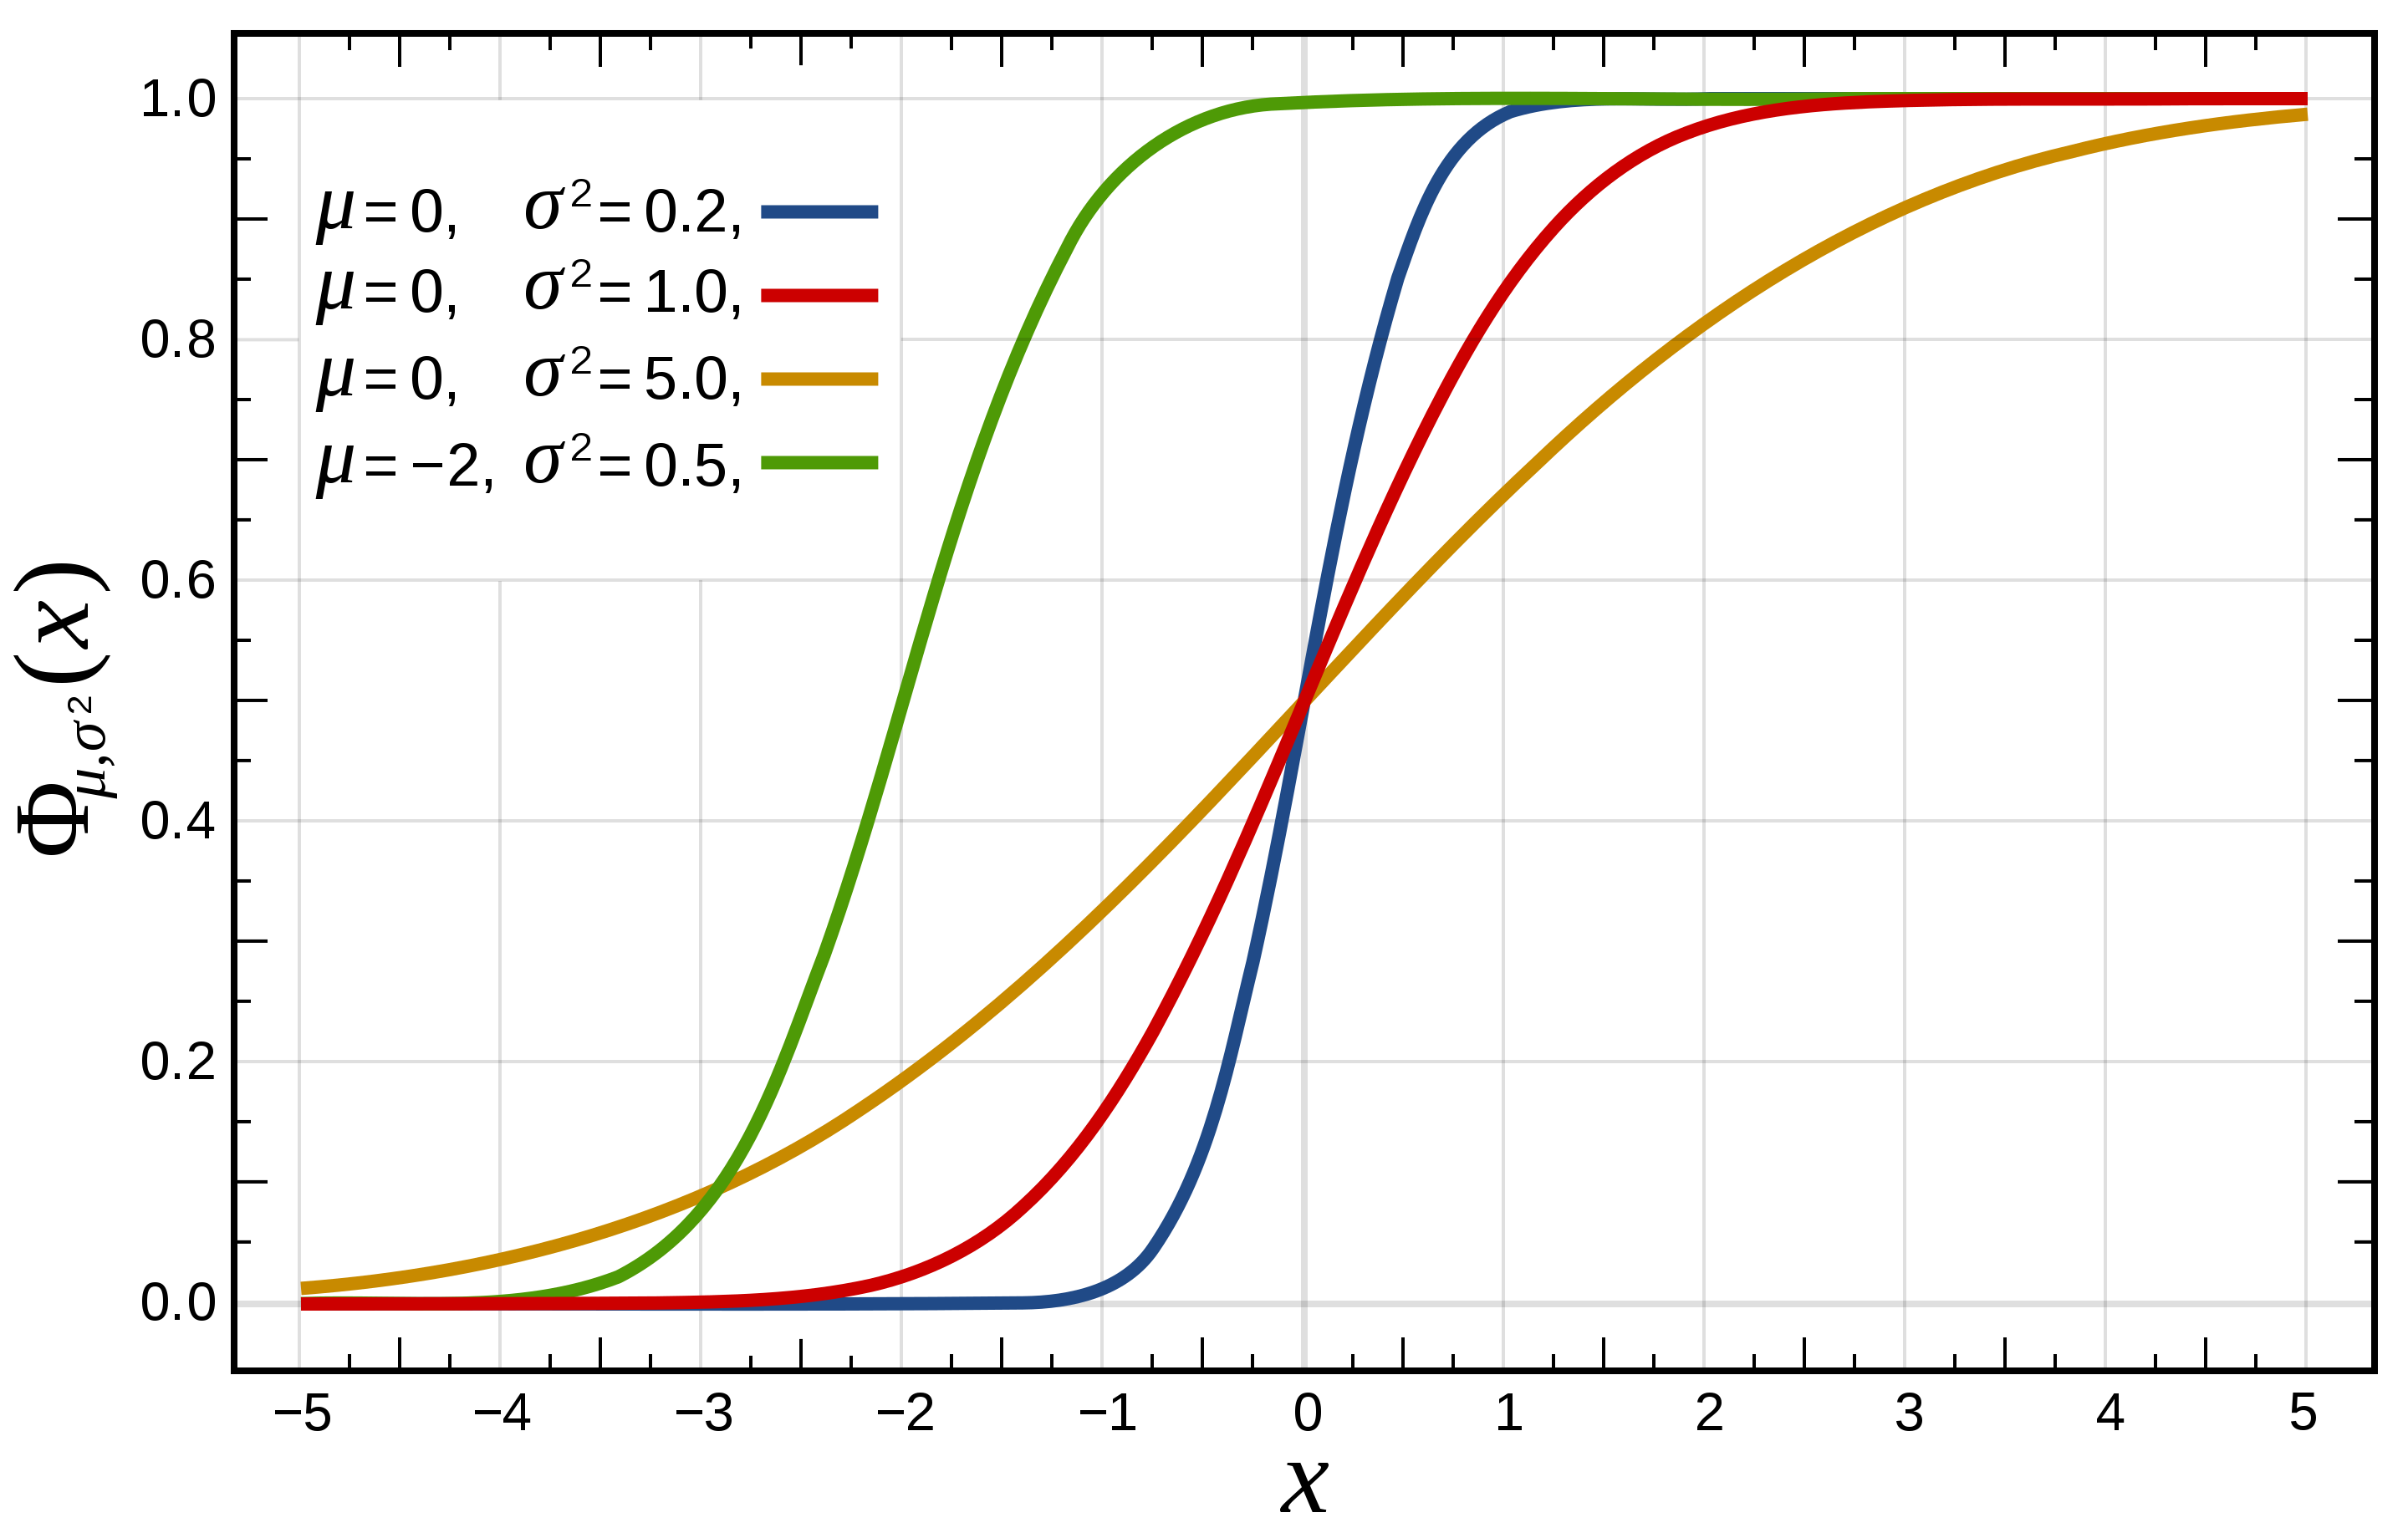
\includegraphics[scale=0.08]{normal_cdf.png}
	\caption[]{Cumulative Distribution Function (CDF) of Normal distribution.}
	\label{fairdiepmf}
	\end{center}
	\end{figure}
	
About 68\% of values drawn from a normal distribution are within one standard deviation $\sigma$ away from the mean $\mu$. About 95\% of the values lie within two standard deviations and about 99.7\% are within three standard deviations. This is known as the 68-95-99.7 rule. 

\begin{figure}[h!]
\begin{center}
	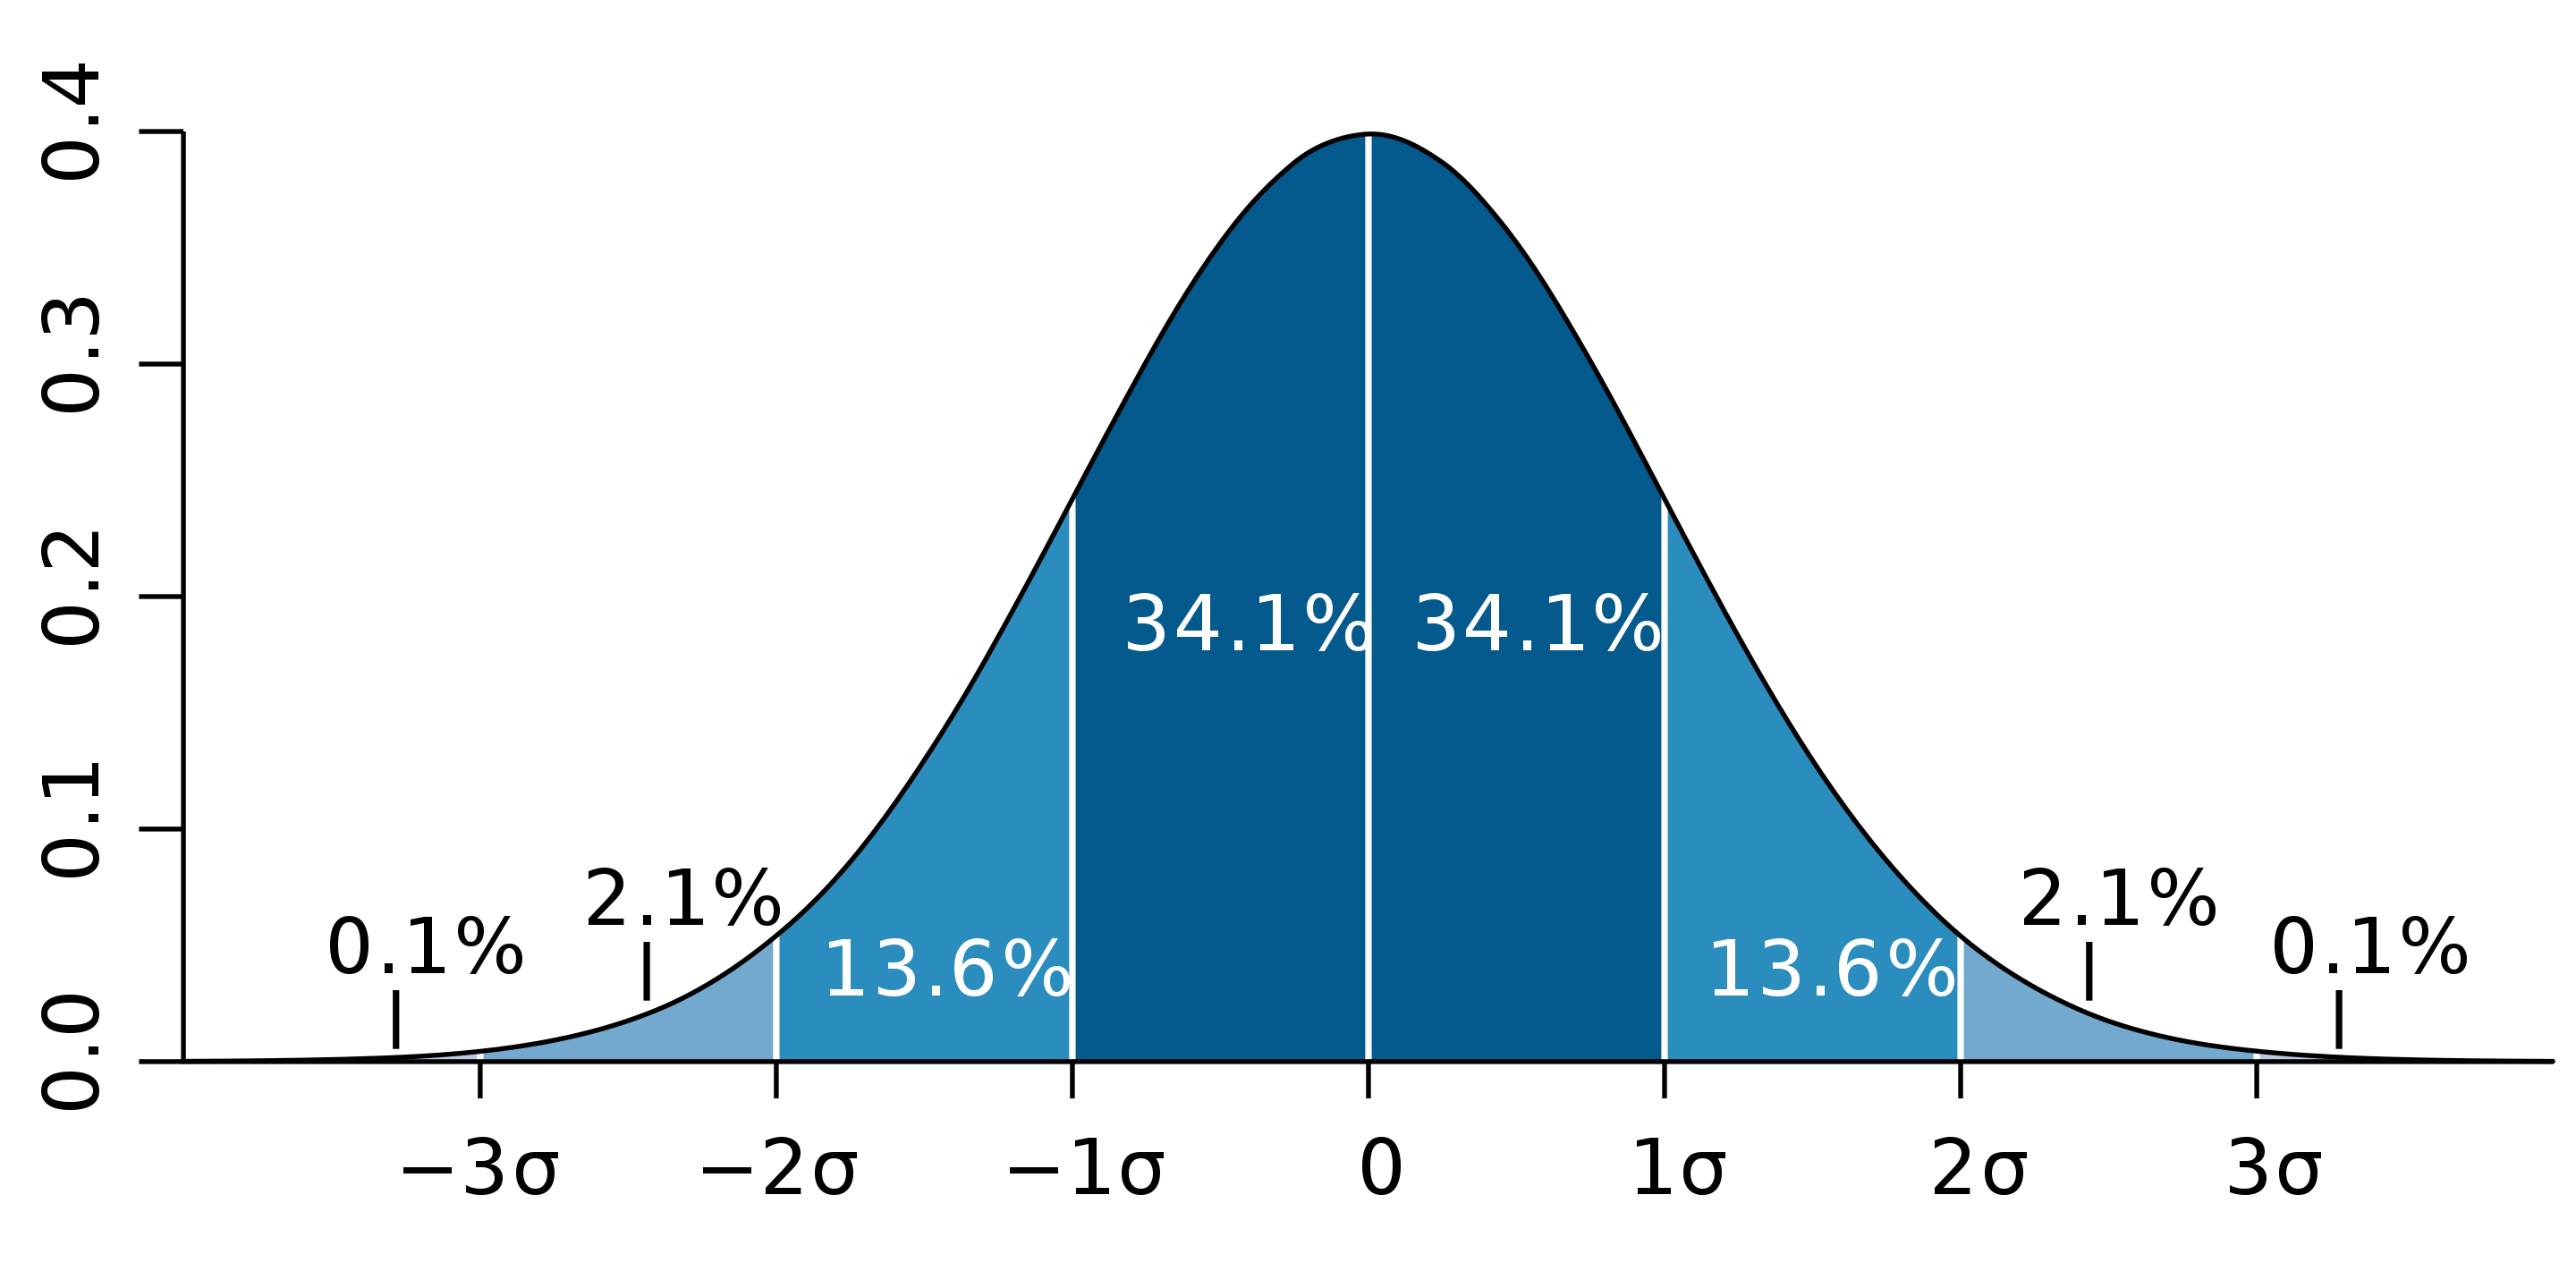
\includegraphics[scale=0.08]{normal_sd.png}
	\caption[]{Normal distribution with standard deviation}
	\label{fairdiepmf}
	\end{center}
	\end{figure}
	

\section{Continuous variable: Exponential Distribution, Exp($\lambda$)}

Poisson process:\\
the timing of the next event is completely independent of when the previous event happened (memoryless).\\
The number of arrivals of a Poisson process in a given amount of time is Poisson Distributed. \\
The \underline{waiting time} between arrivals of a Poisson process is Exponentially Distributed. \\

The Probability Density Function (PDF) of an exponential distribution is:
\begin{eqnarray}
f(x;\lambda) = \begin{cases}
\lambda e^{-\lambda x},             x \geq 0\\
0,      x < 0
\end{cases}
\end{eqnarray}
where $\lambda$ is the rate parameter used in the Poisson Distribution. \\

The Cumulative Distribution Function (CDF) is given by:
\begin{eqnarray}
F(x;\lambda) = \begin{cases}
1 - e^{-\lambda x},             x \geq 0\\
0,      x < 0
\end{cases}
\end{eqnarray}

\begin{figure}[h!]
\begin{center}
	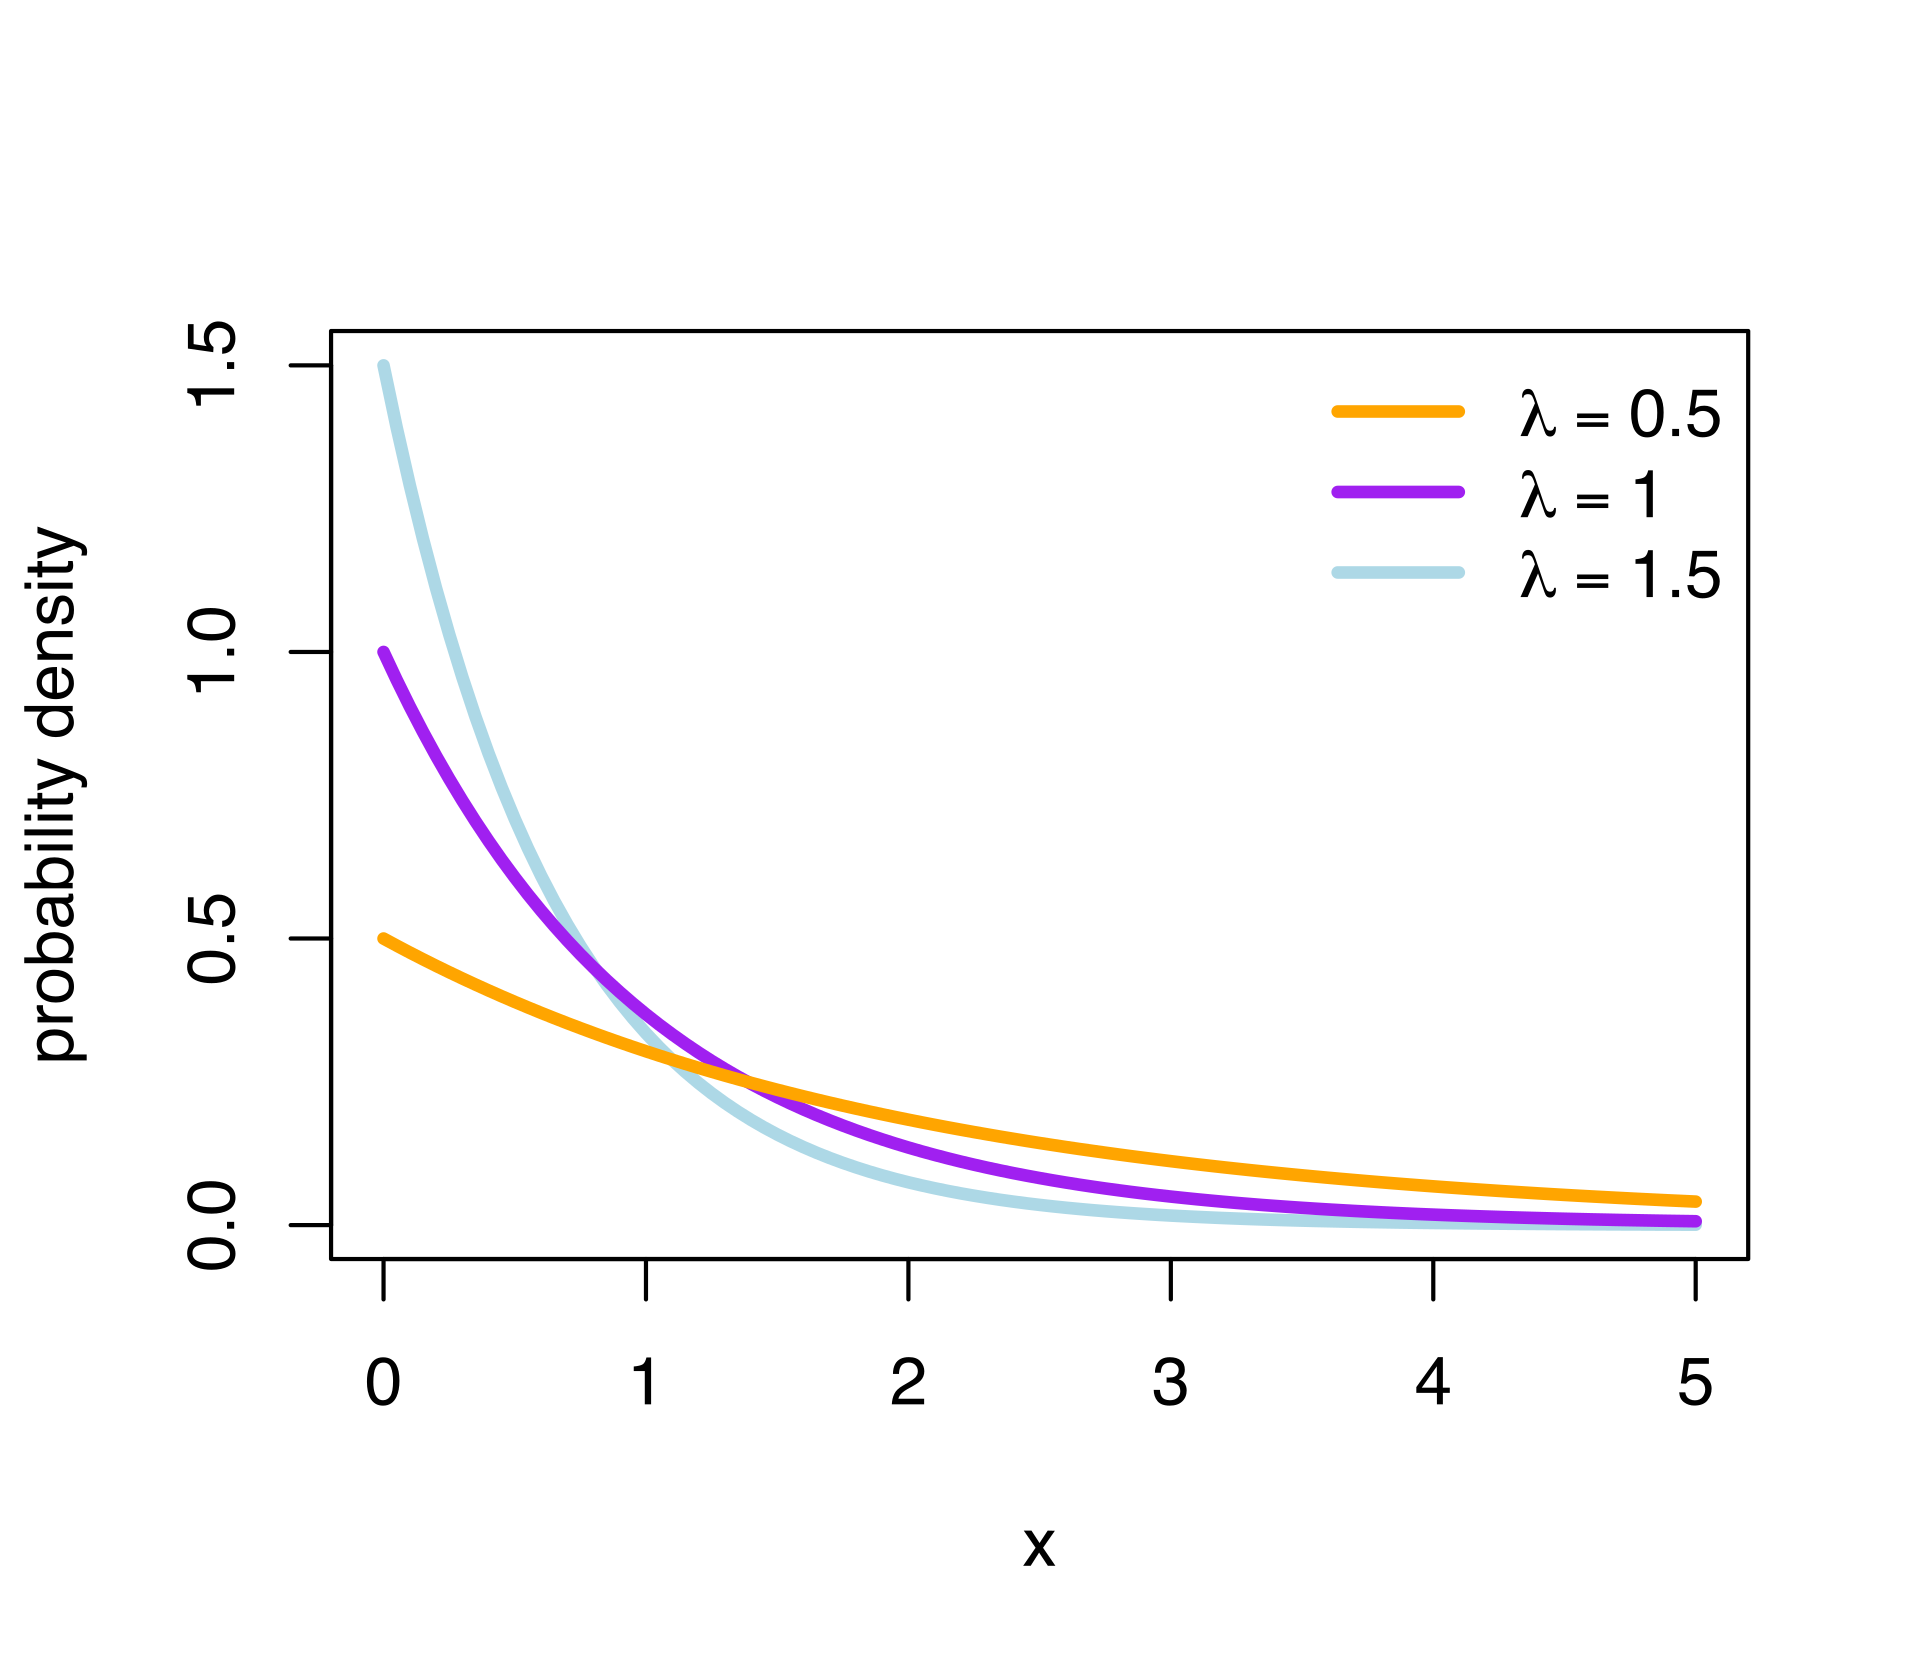
\includegraphics[scale=0.1]{exponential_pdf.png}
	\caption[]{Probability Density Function (PDF) of Exponential Distribution.}
	\label{fairdiepmf}
	\end{center}
	\end{figure}
	
\begin{figure}[h!]
\begin{center}
	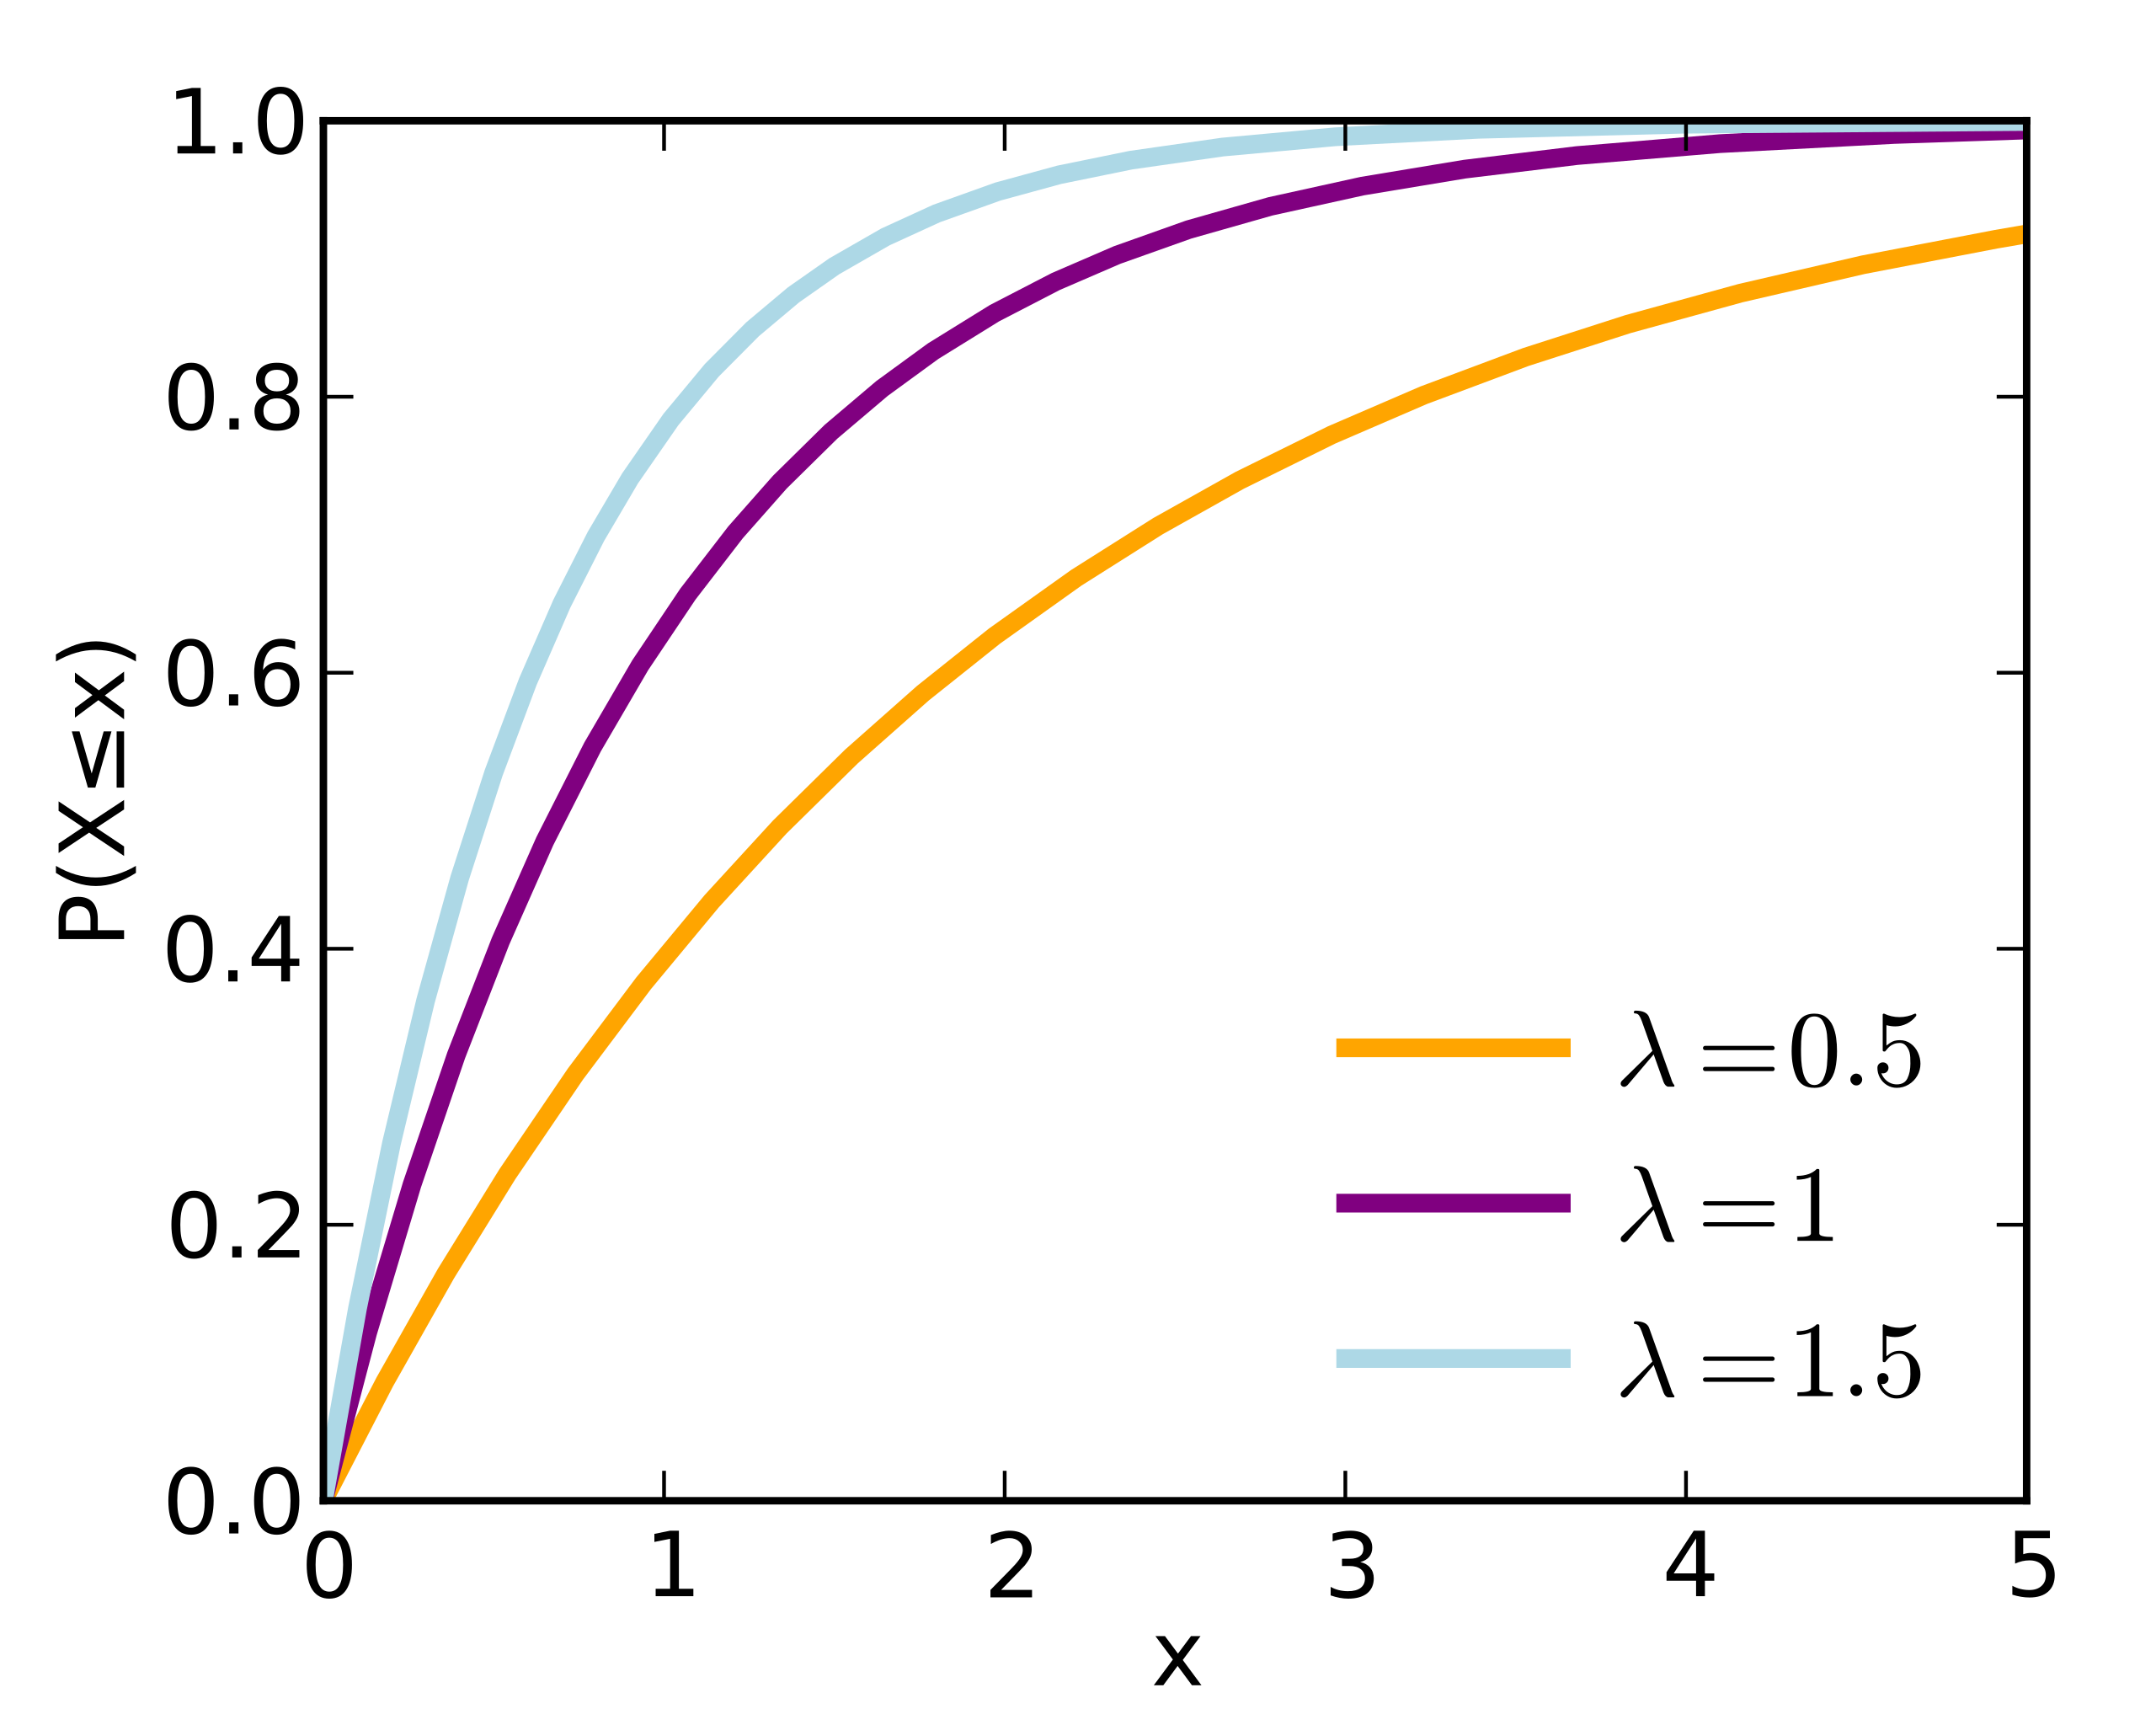
\includegraphics[scale=0.07]{exponential_cdf.png}
	\caption[]{Cumulative Distribution Function (CDF)of Exponential Distribution}
	\label{fairdiepmf}
	\end{center}
	\end{figure}

\section{Continuous variable: Chi-Square Distribution, $\chi^2$}

The chi-square ($\chi^2$) distribution with \underline{k degrees of freedom} is the distribution of a sum of the squares of \underline{k independent standard normal random variables}.  The chi-square distribution is used in the common chi-square chi-square tests for goodness of fit of an observed distribution to a theoretical one. \\

Let's say we have some random variables, each of them are independent standard, normally distributed random variables. Say we have random variable $X_1$:
\begin{eqnarray}
X_1 \sim N(0, 1)
\end{eqnarray}
This variable has mean = 0, variance/standard deviation = 1 and follows Normal Distribution.  \\

Say now we have a new random variable $Q = X_1^2$, i.e. we sample from the distribution of $X_1$ and square whatever number we have. Q will have a chi-square distribution with k = 1 degree of freedom, i.e. $Q \sim \chi^2_1$. If $Q = X_1^2 + X_2^2$ then Q will have a degree of freedom = 2, $Q \sim \chi^2_2$.

\begin{figure}[h!]
\begin{center}
	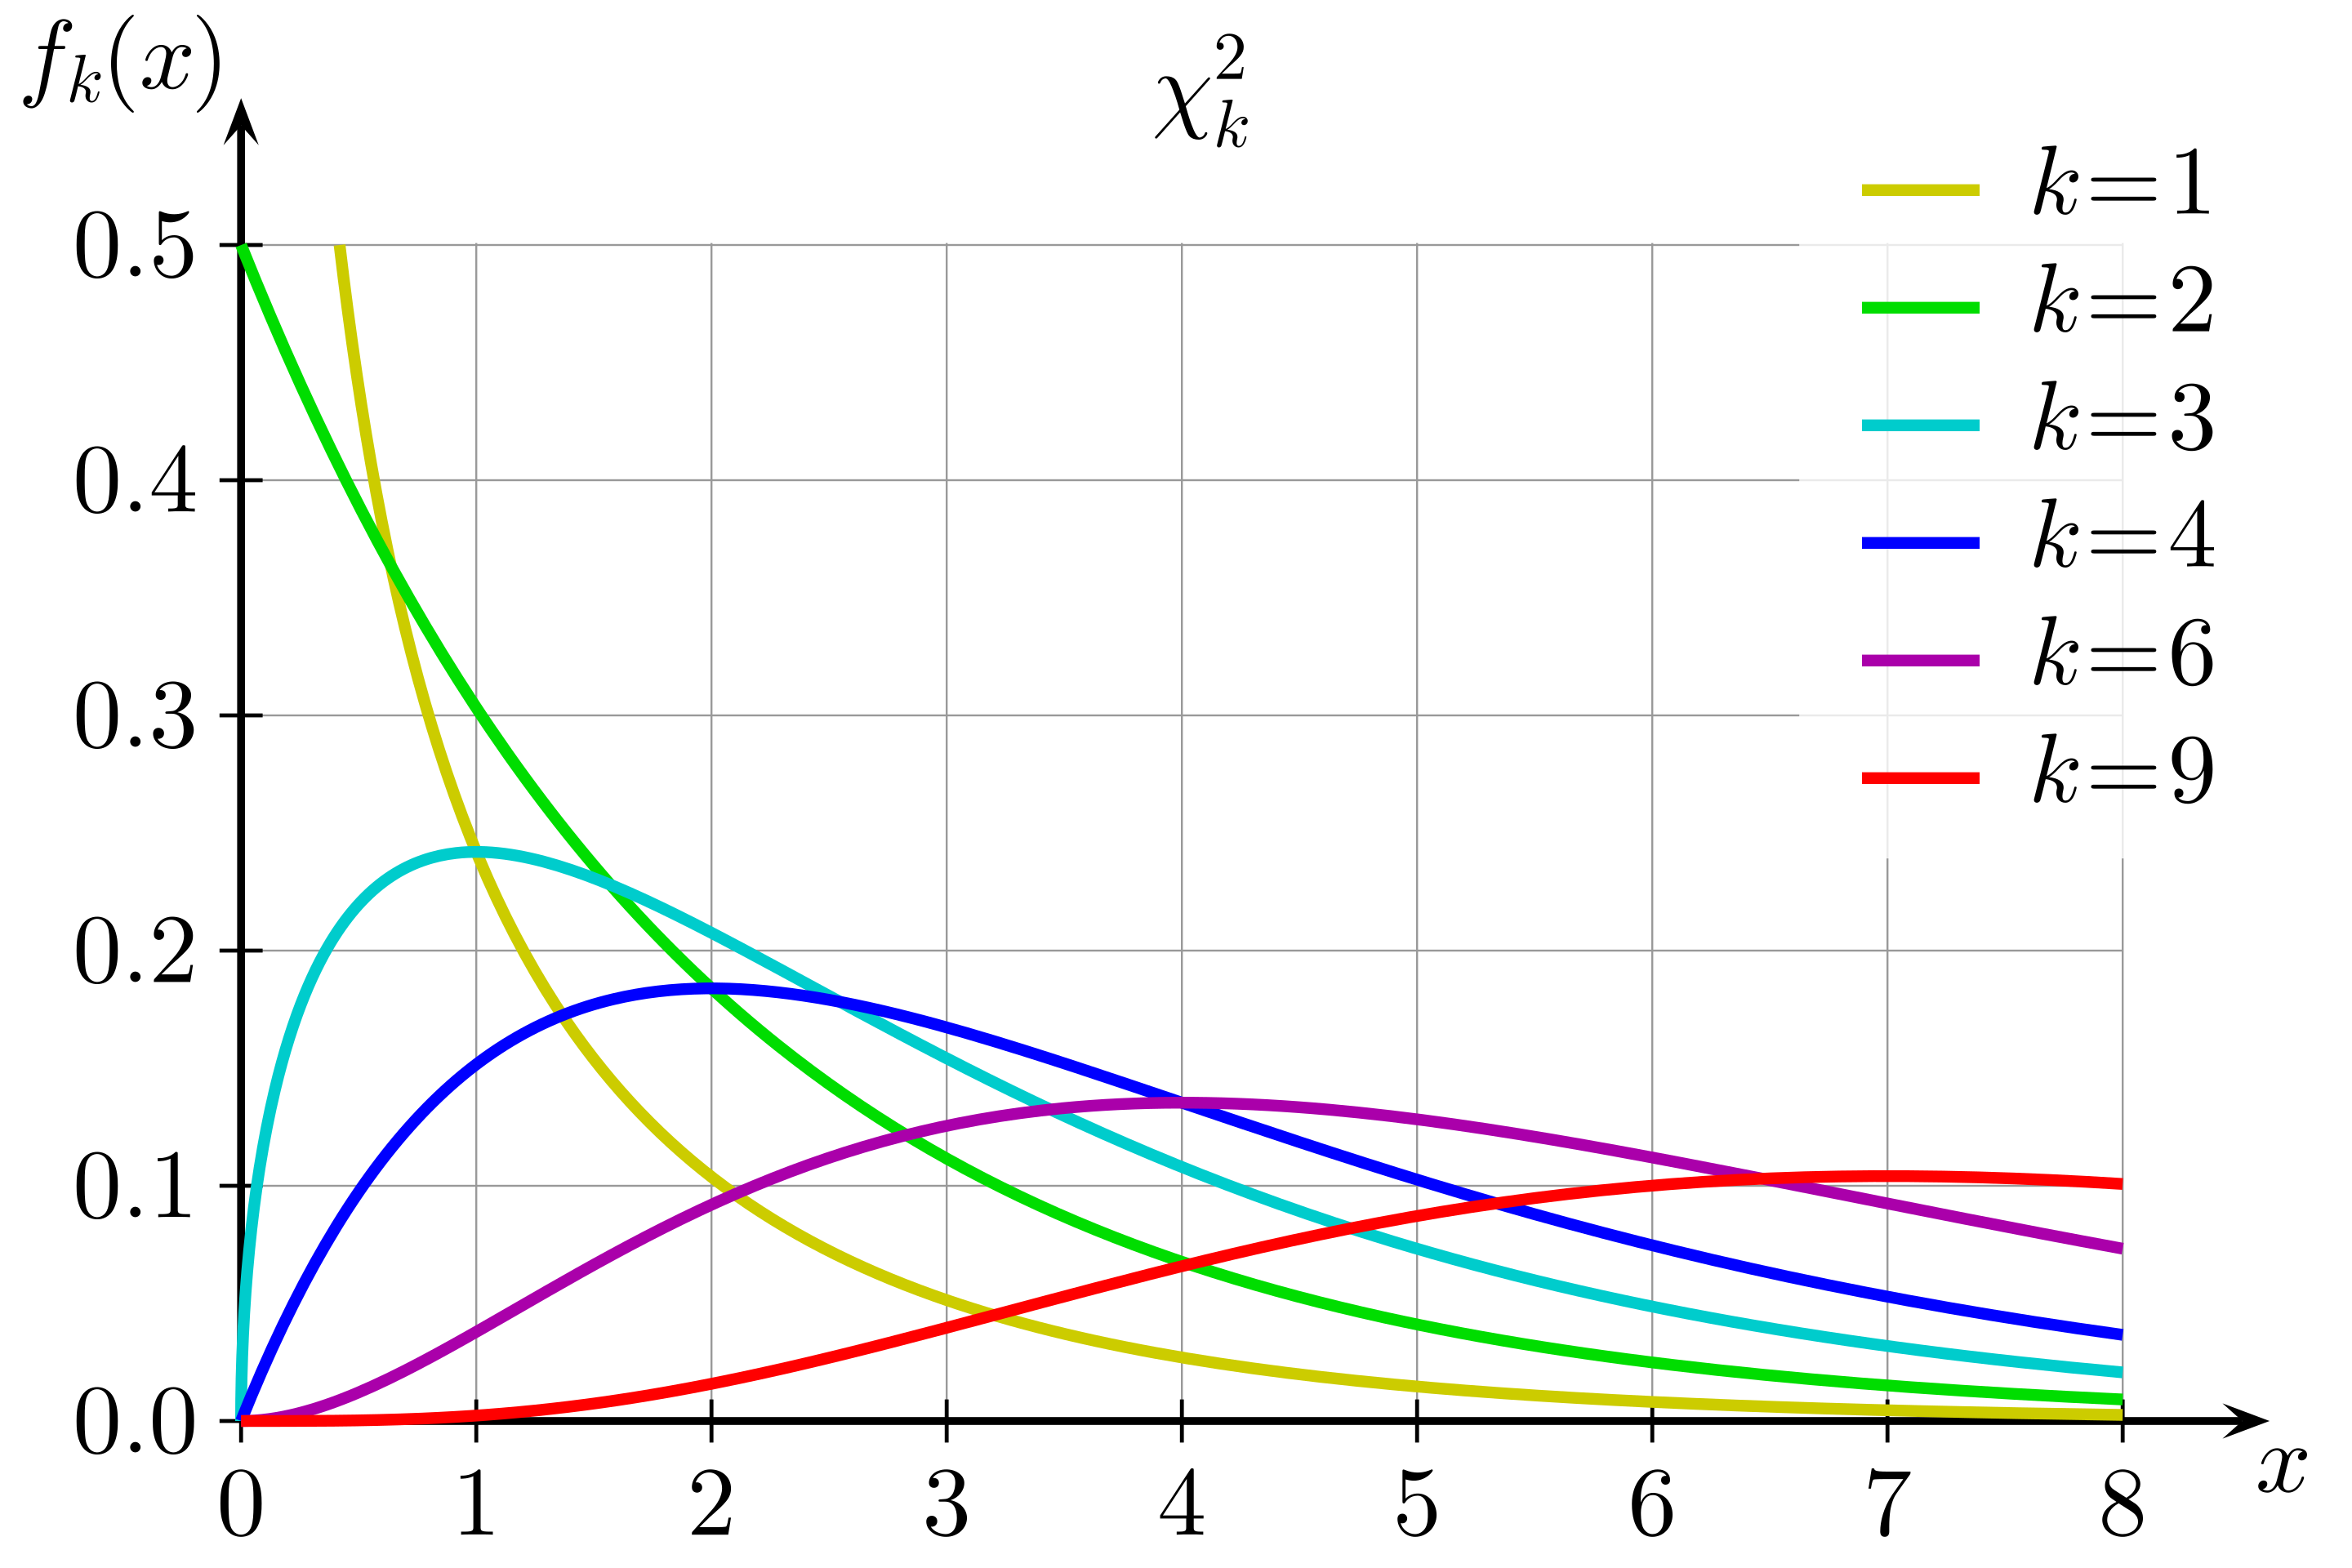
\includegraphics[scale=0.07]{cs_pdf.png}
	\caption[]{Probability Density Function (PDF) of Chi-Square distribution.}
	\label{cspdf}
	\end{center}
	\end{figure}

\begin{figure}[h!]
\begin{center}
	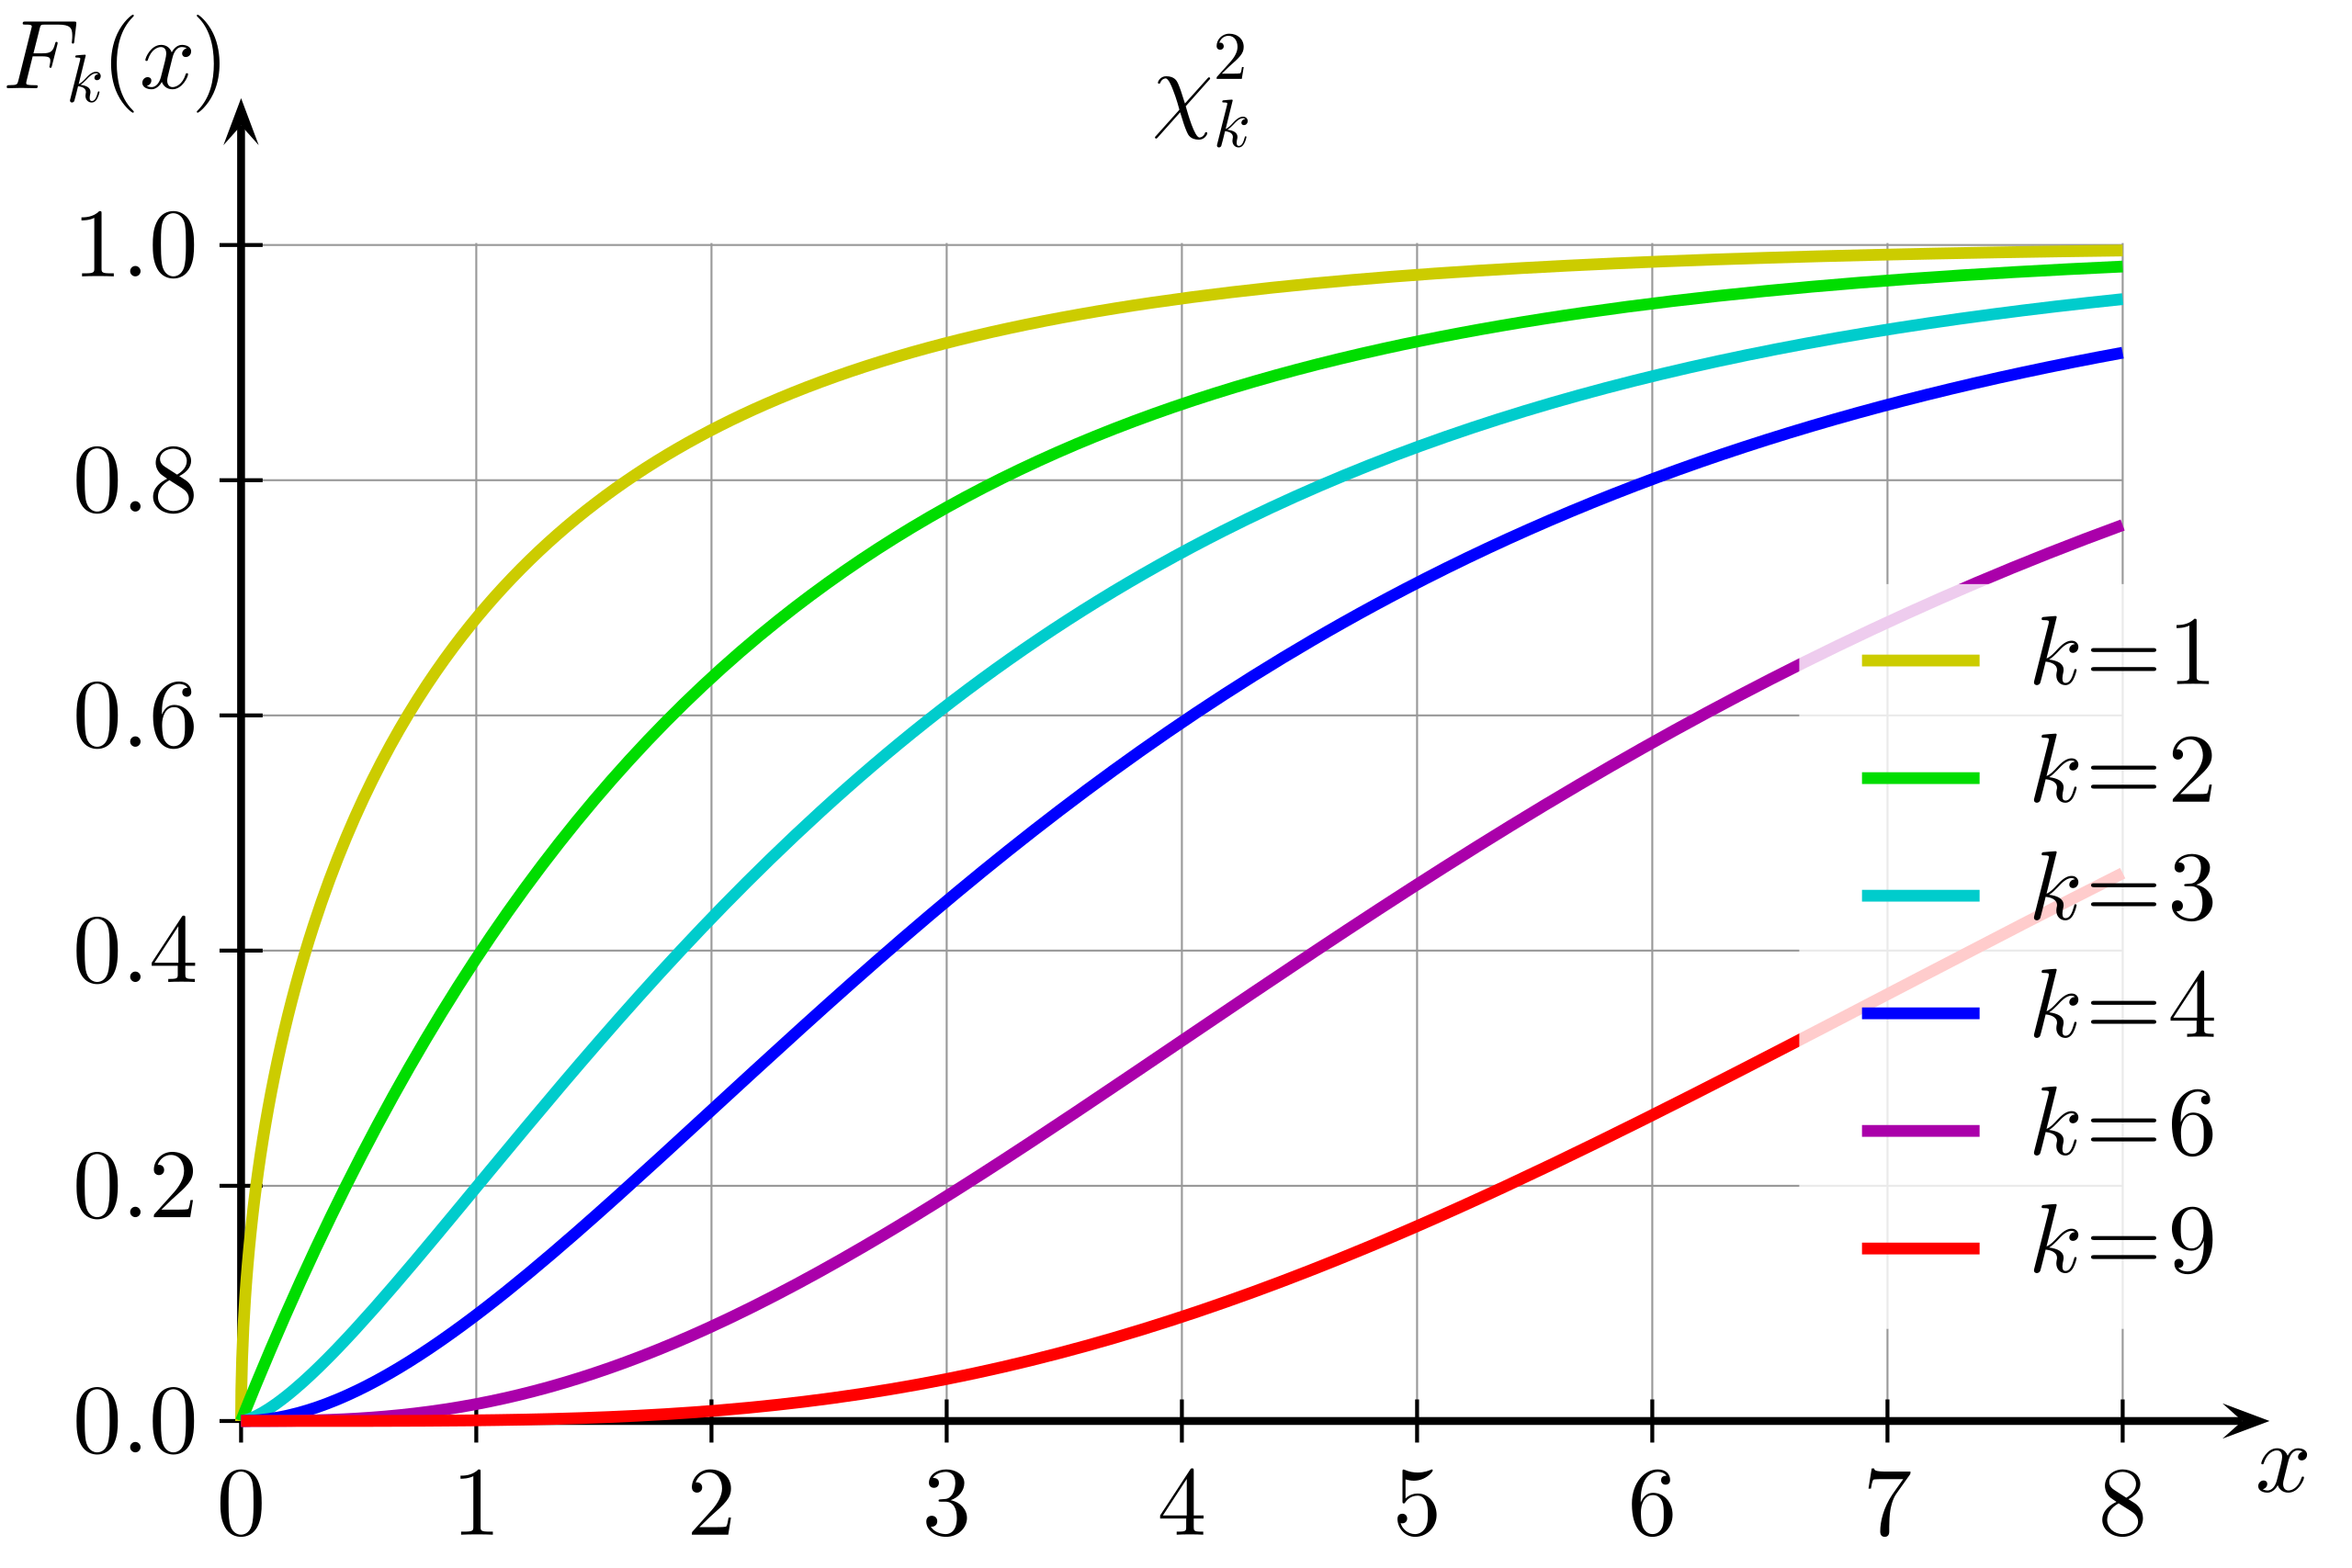
\includegraphics[scale=0.07]{cs_cdf.png}
	\caption[]{Cumulative Distribution Function (CDF) of Chi-Square distribution.}
	\label{cspdf}
	\end{center}
	\end{figure}

The Probability Density Function is shown in Fig.(\ref{cspdf}). For k = 1 the probability is high when x = 0. If we just sample once from $X_1$ we are very likely to get a value that close to 0. 















